% =============================================================================
% Turkish Journal of Engineering (TUJE) -- Research Article
% e-ISSN 2587-1366
% Format follows the official TUJE manuscript template (dergipark.org.tr/en/
% download/journal-file/35111):
%   - Two columns, Cambria font, 10 pt body / 9 pt abstract, single spacing
%   - A4, 1.5 cm margins on all four sides, 0.5 cm first-line paragraph indent
%   - Abstract <= 300 words, no mathematics; 3-5 keywords on the left
%   - Main sections INTRODUCTION / METHOD / RESULTS / DISCUSSION / CONCLUSION:
%     10 pt, bold, ALL CAPS, justified. Second-level headings: left aligned,
%     10 pt, bold, sentence case.
%   - Tables: "Table N. Name", 10 pt title (not bold/italic), 9 pt in-table
%     text, no vertical rules. Figures: "Figure N. Caption", 10 pt, >=400 dpi.
%   - References: numbered [n] citation in text; APA 6 reference-list entries.
% Compile: xelatex tuje_dynamic_fusion.tex (run twice for cross-references)
% =============================================================================
\documentclass[10pt,a4paper,twocolumn]{article}

\usepackage[a4paper,margin=1.5cm,columnsep=0.6cm]{geometry}
\usepackage{fontspec}
\setmainfont{Cambria}
\usepackage{amsmath,amssymb}
\usepackage{booktabs}
\usepackage{array}
\usepackage{multirow}
\usepackage{graphicx}
\usepackage{caption}
\usepackage[hidelinks]{hyperref}
\usepackage{tikz}
\usetikzlibrary{arrows.meta,positioning,calc,shapes.geometric,fit,backgrounds}
\usepackage{enumitem}
\setlist{nosep,leftmargin=1.4em}

\captionsetup{font=small,labelfont=bf,labelsep=period}
\captionsetup[table]{skip=4pt}

\usepackage{titlesec}
\titleformat{\section}{\normalfont\bfseries\upshape}{\thesection.}{0.5em}{\MakeUppercase}
\titleformat{\subsection}{\normalfont\bfseries}{\thesection.\arabic{subsection}.}{0.5em}{}
\titleformat{\subsubsection}{\normalfont\bfseries\itshape}{\thesection.\arabic{subsection}.\arabic{subsubsection}.}{0.5em}{}
\titlespacing*{\section}{0pt}{8pt}{4pt}
\titlespacing*{\subsection}{0pt}{6pt}{3pt}
\titlespacing*{\subsubsection}{0pt}{5pt}{2pt}

\setlength{\parindent}{0.5cm}
\renewcommand{\arraystretch}{1.15}

\setcounter{topnumber}{3}
\setcounter{bottomnumber}{2}
\setcounter{totalnumber}{4}
\setcounter{dbltopnumber}{2}
\renewcommand{\topfraction}{0.92}
\renewcommand{\bottomfraction}{0.7}
\renewcommand{\textfraction}{0.06}
\renewcommand{\floatpagefraction}{0.6}
\renewcommand{\dbltopfraction}{0.92}
\renewcommand{\dblfloatpagefraction}{0.6}

\hyphenation{cross-sectional walk-forward over-fitting calibra-tion soft-max}

% =============================================================================
\begin{document}
\twocolumn[{%
\centering
\rule{\textwidth}{0.4pt}\\[2pt]
{\small Turkish Journal of Engineering \textbar{} \itshape https://dergipark.org.tr/en/pub/tuje \textbar{} \upshape e-ISSN 2587-1366}\\[1pt]
\rule{\textwidth}{0.4pt}\\[12pt]

{\LARGE\bfseries Dynamic Uncertainty-Weighted Fusion for Multi-Source Financial Data:\\[3pt]
A Bayesian Framework for Time-Varying Source Reliability\par}
\vspace{12pt}

{\large Anandkumar Pardeshi\,$^{*1}$\quad Sujata Deshmukh\,$^{2}$\par}
\vspace{8pt}

{\footnotesize\itshape
$^{1}$Fr.\ C.\ Rodrigues Institute of Technology, Department of Computer Science and Engineering, Navi Mumbai, India. anand.pardeshi@fcrit.ac.in\\[1pt]
$^{2}$Fr.\ Conceicao Rodrigues College of Engineering, Department of Computer Engineering, Bandra, Mumbai, India. sujata.deshmukh@frcrce.ac.in\par}
\vspace{8pt}

\begin{minipage}{0.95\textwidth}
\footnotesize
\textbf{Cite this study:} Pardeshi, A., \& Deshmukh, S. (2026). Dynamic uncertainty-weighted fusion for multi-source financial data: A Bayesian framework for time-varying source reliability. \textit{Turkish Journal of Engineering}.
\end{minipage}
\vspace{12pt}

\noindent\fbox{\begin{minipage}{0.96\textwidth}
\fontsize{9}{11}\selectfont
\begin{minipage}[t]{0.27\textwidth}
\raggedright
\textbf{Keywords}\\[3pt]
Multi-source data fusion\\
Bayesian dynamic weighting\\
Uncertainty quantification\\
Data leakage\\
Financial forecasting\\[8pt]
\textbf{Research Article}\\[3pt]
Received\,: \\
Revised\,: \\
Accepted\,: \\
Published\,:
\end{minipage}\hfill
\begin{minipage}[t]{0.66\textwidth}
\raggedright
\textbf{Abstract}\\[3pt]
Multi-source fusion architectures that combine technical, sentiment, and volatility signals routinely assume that each source's reliability is fixed, and a competing line of work proposes weighting each source by a softmax function of its recent prediction uncertainty as the remedy. This proposal is tested here against the authors' own deployed implementation of exactly this mechanism, with the evaluation itself subjected to the same scrutiny as the system under test. Two concrete failure modes surfaced first in the deployed code: the error-feedback loop is never invoked, so weights sit at equal division, and once wired up, the raw formula proved numerically inert at realistic return-forecasting error scales; a scale-normalized variant restores genuine differentiation. With two price-derived sources, technical and volatility, the corrected mechanism showed no significant benefit over static fusion at next-day direction across 44 NSE large-caps, 2018--2026, and a small 20-day-horizon effect vanished under a conviction gate. Adding a third, genuinely independent source -- real US-dollar-to-rupee and crude-oil data -- first appeared to change this picture: an early pass showed dynamic fusion beating static fusion by nine-hundredths of a percentage point, surviving a Bonferroni correction across every comparison in the paper. Auditing the evaluation harness as rigorously as the deployed system had been audited uncovered two independent look-ahead defects behind that number: a timezone misalignment that let the macro features leak same-day information not yet available at prediction time, and an error-feedback loop that updated a day's fusion weights using that same day's own outcome. Correcting both collapses the effect to nine-thousandths of a percentage point with a confidence interval that includes zero. A pre-registered train/test split on the fusion rule's implicit learning-rate parameter recovers no effect either, and further demonstrates the failure mode directly: a parameter value chosen on a selection window shows a positive effect in-sample and a negative point estimate out-of-sample. A parallel analysis on mean squared error, the mechanism's literal design objective, tells the same null story. This mechanism, correctly implemented and evaluated free of look-ahead leakage, shows no reliable advantage over static fusion in any of the eight source configurations, two horizons, or two evaluation metrics tested here -- and the full sequence is reported: how a plausible-looking positive result was manufactured by the evaluation harness, and how it was caught, offered as a reusable checklist for exactly this failure mode in future multi-source fusion work.
\end{minipage}
\end{minipage}}
\vspace{14pt}
}]

% =============================================================================
\section{Introduction}
% =============================================================================

Forecasting systems for equity markets increasingly combine more than one kind of evidence: price and volume history, natural-language sentiment extracted from news, and market-wide risk gauges such as an implied-volatility index. The appeal is straightforward -- each source captures something the others miss, and a system that reads all of them should dominate one that reads only one. What is far less settled is how the sources should be combined, and in particular whether the relative weight given to each source should change over time as market conditions change.

\subsection{Multi-source financial forecasting}

A large and still-growing literature confirms that combining sources helps. Early fusion concatenates raw or engineered features from every source into one input vector before a single model consumes them \cite{moodi2024,mu2023}; late fusion trains one model per source and combines the outputs by averaging, voting, or a learned meta-model \cite{farimani2024,vargas2022}; and hybrid or attention-based fusion lets a neural layer learn, implicitly, how much each modality should matter \cite{liu2019,haryono2023}. Systematic reviews of this space \cite{zhang2022,li2020} agree that fusing sources beats using any single one, and the trend has accelerated as large language models have made high-quality sentiment extraction cheap \cite{jung2024,liu2024llm}.

The definition of a ``source'' keeps expanding, too. Beyond price series and news sentiment, adversarial-learning approaches now fuse structured market data with genuinely heterogeneous alternative data -- web traffic, ownership networks, transaction graphs -- inside a single FinTech pipeline \cite{khuwaja2023}, and the fusion layer itself keeps getting more expressive: normalizing flows have been used to model the joint distribution of sentiment and price signals rather than simply weighting them \cite{tai2022}, Kolmogorov--Arnold network variants have been paired with generative aspect-based sentiment extraction for a tighter coupling between the two modalities \cite{haryono2024}, and sentiment has been folded directly into recommendation-style scoring rather than treated as a separate predictive channel \cite{wang2024spcm}. Recurrent architectures very close to the technical expert examined in this paper -- a GRU consuming endogenous price features alongside exogenous market variables -- remain a standard and independently validated choice for the price-based component of a fusion system \cite{alsheebah2024}, which is one reason this architectural choice is treated as settled rather than something this paper needed to re-litigate.

A separate strand treats combination not as a prediction-fusion problem but as a policy-fusion one: multi-agent and reinforcement-learning formulations let several trading agents, each reading a different signal, arbitrate through a learned policy rather than a weighted-average forecast \cite{lee2007}, and the same idea recurs in adjacent, faster-moving markets -- cryptocurrency price prediction has its own sentiment-fusion literature facing an identical static-weighting critique \cite{parekh2022}, and classical sliding-window and big-data time-series pipelines that predate the fusion literature altogether \cite{chou2018,wang2020tsmining} are still the baseline every fusion paper in this space is implicitly trying to beat. None of these variants, whatever their sophistication, revisit the assumption this paper is concerned with: that once a fusion layer -- of any of the kinds above -- is trained, the relative trust it places in each source is fixed for the life of the model.

\subsection{The static-fusion problem}

Almost every fusion scheme in this literature, however, fixes the relative importance of each source once training finishes. A concatenated feature vector, an averaged ensemble, and a learned attention layer all encode a relationship between sources that is estimated once over a training window and then applied unchanged at every subsequent prediction. This sits awkwardly next to a basic fact about markets: their regimes change. Technical indicators tend to be informative in a trending, low-noise market and much less so during a sentiment-driven shock: Bacco et al.\ \cite{bacco2024} explicitly study prediction under high uncertainty but still fuse with a fixed architecture. Zhang et al.'s review \cite{zhang2022} names ``dynamic integration of different data sources based on their time-varying predictive power'' as an open problem, not a solved one.

The natural fix is to make the fusion weights a function of how much each source's recent predictions can be trusted -- a Bayesian-flavored idea in which a source's own recent error variance stands in for its momentary reliability, and the weights update as that reliability changes. A softmax over negative per-source uncertainty,
\[
w_i = \frac{\exp(-\sigma_i^2)}{\sum_j \exp(-\sigma_j^2)},
\]
is an obvious and appealing instantiation: low recent error means high confidence means high weight, and the assignment updates every time a new outcome is observed.

\subsection{Dynamic expert weighting beyond finance}

The idea of combining several predictors by a weight that adapts to their recent track record did not originate in finance, and it is worth situating the finance-fusion literature inside the older and more general theory of combining experts, because that theory already anticipates the failure mode reported in Section 3. Mixture-of-experts models learn a gating network that routes each input to the most competent sub-model \cite{jacobs1991}. Bayesian model averaging treats the weight on each candidate model as its posterior probability given the data seen so far, updated by Bayes' rule every time new evidence arrives \cite{hoeting1999}. Closest to the mechanism examined here, the Hedge algorithm and its relatives from online learning theory assign each expert a weight proportional to $\exp(-\eta \cdot \text{loss}_i)$, where $\eta$ is a learning-rate parameter chosen deliberately, in full knowledge that the wrong choice of $\eta$ makes the multiplicative-weights update either too flat to discriminate between experts or too sharp to be stable \cite{freundschapire1997,cesabianchi2006}. The softmax-uncertainty rule in Section 1.2 is, formally, a Hedge-style update with $\eta$ implicitly fixed to $1$ rather than tuned to the loss scale of the task -- which is exactly the condition Section 2.1.2 shows breaks down at the error scales financial returns actually produce, and exactly the problem the scale-normalization introduced in that section is designed to correct. Reinventing a learning-rate parameter was not the original goal; finding that the deployed formula was missing one is itself informative about why a mathematically motivated fusion rule can under-perform in practice.

\subsection{What this paper does differently}

The idea above is not hypothetical here. It has already been implemented, feature set and formula both, in the authors' own deployed multi-source forecasting system (an NSE-India equity forecasting platform with a technical expert, a sentiment expert, and a volatility expert combined by exactly this softmax rule). That creates an unusual opportunity: rather than proposing the mechanism and then simulating whether it would probably help, the running system itself can be audited, checked for whether it actually works as intended, fixed where it does not, and measured on real market data. All three were done -- and, in the course of the third, the same auditing discipline had to be turned on the evaluation code as well, not only on the system it was evaluating, after an early result that looked like a genuine positive turned out to be manufactured by two defects in how it had been scored, not by the mechanism itself. The full sequence is reported: the original architecture defects, the apparent effect, the two evaluation-harness defects that produced it, and the corrected, leak-free result -- because a paper that stops one audit early is not meaningfully more honest than one that never started.

Section 2 describes the deployed architecture, the two concrete problems found in it, the real data and protocol used for each empirical study, and the two further defects found in the evaluation harness together with how the fix was made and stress-tested. Section 3 reports what every study actually found, leak-free throughout. Section 4 discusses why a mathematically correct uncertainty-softmax can still behave like a static average once realistic error scales are inserted into it, why an apparently robust effect can be a data-pipeline artifact rather than a property of the mechanism, and what both imply for the wider claim that dynamic fusion is worth the added complexity. Section 5 concludes.

% =============================================================================
\section{Method}
% =============================================================================

\subsection{The deployed architecture under test}

The system under study assigns one small model to each of three sources -- a technical expert reading 19 OHLCV-derived indicators (moving averages, RSI, MACD, ATR, volume ratio, price-to-moving-average deviations, overnight gap) over a 30-day lookback; a sentiment expert reading an 8-feature summary of multi-source news sentiment (combined score, confidence, per-source sentiment, source availability, article count); and a volatility expert reading 3 features derived from India's implied-volatility index (VIX level, VIX-to-20-day-moving-average ratio, and the stock's own 20-day realized volatility). Each expert predicts next-day raw return. Each expert also keeps a trailing window of its last 10 squared prediction errors and reports their mean as its own uncertainty $\sigma_i^2$; the three predictions are then combined by the softmax rule in Section 1.2, and the combined forecast is what a downstream trading decision would see. Every part of this description -- the feature lists, the 10-day window, the formula -- is read directly from the deployed source, not paraphrased from a specification document, because the specification and the code agreed once checked directly.

\begin{figure*}[t]
\centering
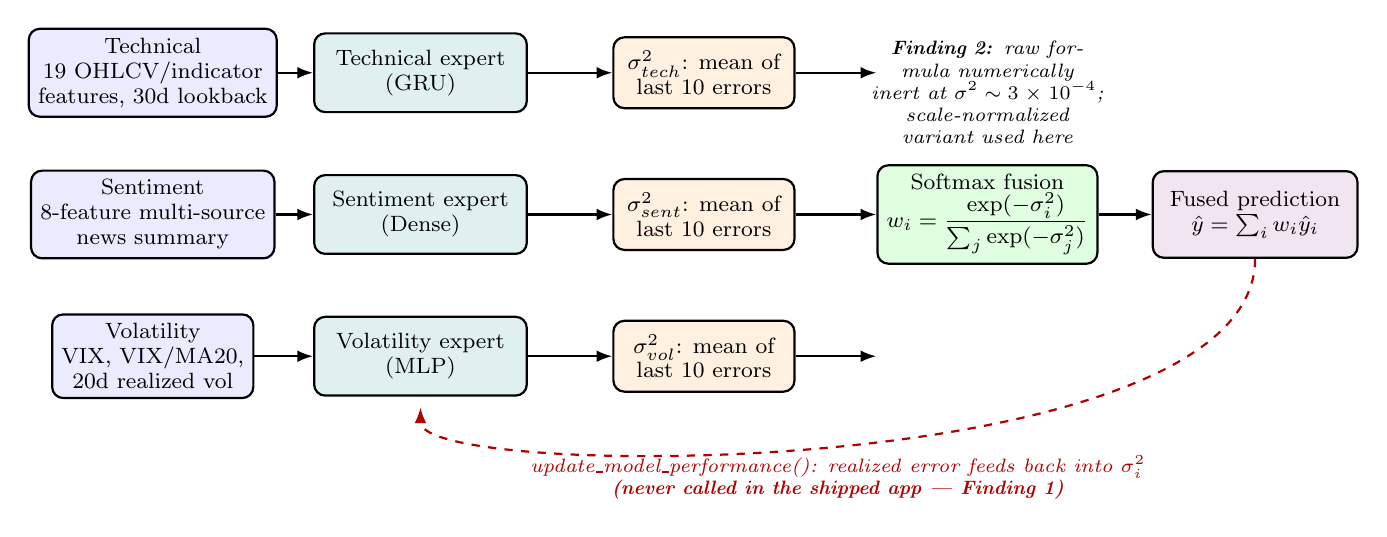
\begin{tikzpicture}[
  font=\fontsize{8}{9}\selectfont,
  src/.style={draw, rounded corners, fill=blue!8, minimum width=2.5cm, minimum height=0.9cm, align=center, thick},
  exp/.style={draw, rounded corners, fill=teal!12, minimum width=2.7cm, minimum height=1.0cm, align=center, thick},
  unc/.style={draw, rounded corners, fill=orange!12, minimum width=2.3cm, minimum height=0.9cm, align=center, thick},
  fus/.style={draw, rounded corners, fill=green!12, minimum width=2.6cm, minimum height=1.1cm, align=center, thick},
  lbl/.style={font=\fontsize{7}{8}\selectfont\itshape}
]
\node[src] (tech) at (0,3.6) {Technical\\19 OHLCV/indicator\\features, 30d lookback};
\node[src] (sent) at (0,1.8) {Sentiment\\8-feature multi-source\\news summary};
\node[src] (vol)  at (0,0)   {Volatility\\VIX, VIX/MA20,\\20d realized vol};

\node[exp] (etech) at (3.4,3.6) {Technical expert\\(GRU)};
\node[exp] (esent) at (3.4,1.8) {Sentiment expert\\(Dense)};
\node[exp] (evol)  at (3.4,0)   {Volatility expert\\(MLP)};

\node[unc] (utech) at (7.0,3.6) {$\sigma^2_{tech}$: mean of\\last 10 errors};
\node[unc] (usent) at (7.0,1.8) {$\sigma^2_{sent}$: mean of\\last 10 errors};
\node[unc] (uvol)  at (7.0,0)   {$\sigma^2_{vol}$: mean of\\last 10 errors};

\node[fus] (softmax) at (10.6,1.8) {Softmax fusion\\$w_i=\dfrac{\exp(-\sigma_i^2)}{\sum_j\exp(-\sigma_j^2)}$};
\node[fus, fill=violet!10] (out) at (14.0,1.8) {Fused prediction\\$\hat y=\sum_i w_i\hat y_i$};

\foreach \a/\b in {tech/etech, sent/esent, vol/evol, etech/utech, esent/usent, evol/uvol}
  \draw[-{Latex[length=2mm]}, thick] (\a) -- (\b);
\draw[-{Latex[length=2mm]}, thick] (utech) -- (softmax.north west|-utech);
\draw[-{Latex[length=2mm]}, thick] (usent) -- (softmax.west);
\draw[-{Latex[length=2mm]}, thick] (uvol)  -- (softmax.south west|-uvol);
\draw[-{Latex[length=2mm]}, thick] (softmax) -- (out);

% Feedback loop (Finding 1: dead in the shipped app)
\draw[-{Latex[length=2mm]}, thick, red!70!black, dashed]
  (out.south) .. controls (14.0,-1.6) and (3.4,-1.6) .. (3.4,-0.65)
  node[midway, below, lbl, red!70!black, align=center]
  {update\_model\_performance(): realized error feeds back into $\sigma_i^2$\\\textbf{(never called in the shipped app --- Finding 1)}};

\node[lbl, align=center, text width=3.6cm] at (10.6,3.35) {\textbf{Finding 2:} raw formula numerically\\inert at $\sigma^2\!\sim\!3\times10^{-4}$;\\scale-normalized variant used here};

\end{tikzpicture}
\caption{The deployed Dynamic Fusion architecture under test. Solid arrows are the real, active data path; the dashed red arrow is the error-feedback connection that Section~2.1.1 finds is never invoked in the shipped interactive tool, so $\sigma_i^2$ never updates and $w_i$ collapses to $1/3$ for every source. Section~2.1.2 identifies a second problem in the softmax step itself.}
\label{fig:arch}
\end{figure*}

\subsubsection{Finding 1: a feedback loop that is never closed}

The uncertainty each expert reports is only ever updated by one function, which appends the latest squared error to that expert's trailing window. In the interactive tool that runs this architecture today, that function is never called inside the loop that produces predictions -- predictions are generated, but the realized outcome that would let each expert judge its own recent accuracy is never fed back in. The practical consequence is simple: every expert's trailing-error window stays empty for the life of the session, its default (maximum) uncertainty value never updates, and the softmax over three identical uncertainties collapses to exactly equal weight, $w_i = 1/3$, on every single prediction the tool has ever produced. The dynamic mechanism is present in the code and absent from its behavior.

\subsubsection{Finding 2: a formula that is numerically inert at realistic scale}

Closing that loop is a small code change, made here, with the architecture re-run using real, continuously updating errors. A second problem then appeared. Next-day equity returns are small, so a competent model's squared error sits in the neighborhood of $\sigma^2 \approx 3\times 10^{-4}$ or smaller. In that regime, $\exp(-\sigma^2) \approx 1 - \sigma^2$, a first-order approximation accurate to within a part in $10^{7}$ -- which means that even a source whose error is, say, twice as large as another's produces a softmax numerator different from its rival's by a few parts in $10^4$. The formula is not wrong; it is simply calibrated for a different numeric regime than the one financial returns live in, and applied literally it barely distinguishes a reliable source from an unreliable one. This is addressed with a scale-normalized variant, $w_i \propto \exp(-\sigma_i^2/\tau_t)$, where $\tau_t$ is the mean of the sources' current uncertainty estimates on day $t$ -- a simple rescaling that makes the softmax exponent order-one regardless of the task's absolute error scale, chosen because it requires no extra hyperparameter beyond what the mechanism already tracks.

\subsection{Study 1: long-horizon, real, two-source evaluation}

To test whether the corrected mechanism earns its complexity, an offline, statistically powered re-implementation was built using the identical feature sets and the identical fusion mathematics described above. The two deep networks (GRU for the technical expert, MLP for the volatility expert) were replaced with ridge regression on the same features, refit quarterly on an expanding window, because retraining two neural networks on every quarter across 44 tickers and 8+ years is computationally prohibitive and does not change the object under test -- the fusion rule itself. The sentiment expert could not be included at this scale (Section 2.3 explains why) so Study 1 evaluates the two sources with genuine multi-year history: technical and volatility.

\textit{Data.} All data are real, sourced from Yahoo Finance via the \texttt{yfinance} API: daily OHLCV for the 45 NIFTY-50 constituent tickers used by the deployed system's own cross-sectional model, 2016-01-01 to 2026-07-16 (one ticker, TATAMOTORS.NS, was excluded after a corporate-action delisting made the symbol unresolvable over the full window, leaving 44 tickers), and the India VIX index (\texttt{\^{}INDIAVIX}) over the same span. Technical features (moving averages, RSI, MACD, ATR, volatility, volume ratio, price-to-MA deviation, gap) were computed with the same formulas as the deployed indicator library. No row, price, or feature in this dataset is synthesized.

\textit{Protocol.} All 44 tickers were pooled into a single panel (111,449 ticker-day rows after feature construction), and a quarterly expanding-window walk-forward was run: at the start of each calendar quarter from 2018Q1 to 2026Q3, both experts are refit on all real data available before that quarter, then used, frozen, to predict every trading day within it. Prediction begins in 2018 to guarantee at least two full years of real training history behind every forecast. On each trading day, the cross-sectional mean squared error of each expert (averaged across whichever of the 44 tickers traded that day) becomes that day's realized-error observation, appended to a 10-observation trailing window per expert -- the same window length used in the deployed code -- from which next-day's dynamic weights are computed. This produces 2,088 real out-of-sample trading days.

\textit{Compared strategies.} (i) Technical expert alone; (ii) volatility expert alone; (iii) static equal-weight fusion ($w=0.5/0.5$, representing the as-shipped default behavior under Finding 1); (iv) dynamic fusion with the raw formula; (v) dynamic fusion with the scale-normalized formula of Section 2.1.2. All five are scored on the same real, held-out days -- nothing is refit or peeked at out of order.

\subsection{Study 2: a short, real, three-source case study}

Reconstructing years of genuine historical news sentiment at daily resolution was not possible within the scope of this study: the project's own real news pipeline uses Yahoo Finance's news endpoint as its only source (a deliberate choice after GDELT proved unusable), and that endpoint returns only a ticker's most recent handful of stories, not an archived history. Rather than substitute a proxy or a simulated sentiment series -- which would have violated the evidentiary standard set for this paper -- a second, smaller, fully real study was run over whatever genuine sentiment history is actually retrievable today.

\textit{Data.} Every available real headline (title, summary, publication timestamp) was pulled for 13 liquid large-cap NSE tickers via the same endpoint the deployed system uses, yielding 130 real headlines spanning 2025-09-29 to 2026-07-18. Each headline was scored by the production sentiment model itself -- \texttt{ProsusAI/finbert}, called through the same function (\texttt{analyze\_sentiment}) and the same bullish/bearish keyword-override rule used in the live system -- producing a genuine label and confidence per headline, converted to a signed value (positive confidence, negative confidence, or zero for neutral). Headlines were mapped to the next real NSE trading day using each ticker's own trading calendar (a headline published after 15:30 IST, or on a non-trading day, rolls forward to the next session), then aggregated per ticker-day into the same 8-feature sentiment summary the deployed sentiment expert consumes (mean, dispersion, positive/negative fraction, and maximum of the signed scores). This produced 88 real ticker-day events with at least one scored headline, each attached to its real realized next-day return and to the same technical- and volatility-expert predictions used in Study 1 for that ticker and date.

\textit{What this study can and cannot show.} With 88 events this is a descriptive case study, not a second statistically powered test. A plain Pearson correlation between real sentiment and real next-day return is reported, an in-sample linear calibration of a sentiment-to-return mapping (there is not enough data for a held-out split), and the fusion mechanism's actual computed behavior -- weights, predictions, accuracy -- when driven by these real three-source events in date order. No claim of out-of-sample predictive significance is made from this sample.

\subsection{Study 3: a longer, conviction-gated horizon}

Study 1 asks the fusion mechanism to distinguish sources at next-day direction, a target this project's own prior work has repeatedly found to carry no exploitable single-name edge beyond drift -- which makes it an unfair arena for judging a \emph{weighting} rule, since there may be too little genuine structure at that horizon for any weighting of these two sources to expose. A fairer test asks the same question where a real, if modest, edge is independently known to exist: a longer horizon, evaluated only on the subset of predictions the system itself flags as high-conviction, mirroring the 30-day conviction-gated design already validated elsewhere in this codebase.

\textit{Design.} Study 1's identical real data, identical features, identical quarterly walk-forward, and identical fusion mathematics were re-run, changing only the prediction target from next-day return to 20-trading-day forward log return, and adding a conviction gate that retains only the top 20\% of predictions by the magnitude of the (static) combined forecast, evaluated separately from the full, ungated sample. Because a 20-day-ahead outcome is not knowable until 20 trading days after the prediction is made, the uncertainty tracker's trailing window is fed with a 20-day lag -- an error observed today is 20 trading days stale by construction, exactly matching the latency a live system would face and preventing any look-ahead into the fusion weights themselves.

\textit{Why the significance test changes.} Forecast windows 20 days apart overlap on 19 of their 20 days, so consecutive observations are strongly autocorrelated and a naive day-by-day bootstrap would understate the true uncertainty of any comparison. A block bootstrap is therefore used, with a block length equal to the horizon (20 trading days), resampling contiguous 20-day chunks of the daily accuracy-difference series rather than individual days -- the standard correction for exactly this kind of overlap.

\subsection{Study 4: a genuinely differentiated third source}

Studies 1 and 3 use only technical and volatility experts, and both are derived from the same underlying price process -- a stock's own OHLCV history and an implied-volatility index computed from options on that same market. Section 4.1 raises the possibility that this is a weak test of the fusion mechanism specifically because the two sources have little reason to disagree about their own reliability at any given moment. To test that directly, a third real source that is not derived from ticker-level price data at all is added here: a macro/FX/commodity expert built from USD/INR (\texttt{INR=X}) and WTI crude oil (\texttt{CL=F}), using the exact feature convention (1-day and 5-day log returns, clipped to $\pm0.2/\pm0.4$) this codebase already uses elsewhere for macro features, so nothing about this source's construction is novel to this paper. Both series have deep, genuine multi-year yfinance history, and both are plausible drivers of Indian equity returns through import costs, energy-sector margins, and foreign-flow sensitivity to the rupee \cite{chenrollross1986}.

\textit{Design.} Study 1's next-day protocol and Study 3's 20-day conviction-gated protocol are repeated exactly, with one change: three experts (technical, volatility, macro) are fit and fused instead of two, using the same quarterly expanding-window walk-forward, the same 44 real tickers, the same scale-normalized softmax now normalized over three sources, and the same 20-day-lagged pending queue for the longer horizon. Static fusion is now a three-way equal weight ($1/3$ each). This produces two comparisons: one at next-day horizon (comparable to Study 1, but with the third source added) and one at the 20-day, conviction-gated horizon (comparable to Study 3, but with the third source added).

\subsection{A self-audit of Study 4's own evaluation harness}
\label{sec:leakaudit}

An early pass through this protocol produced what looked like the paper's cleanest result: dynamic fusion beating static three-way fusion by nine-hundredths of a percentage point at next-day horizon, comfortably past every significance threshold used elsewhere in this paper. Sections 2.1.1 and 2.1.2 had already found two defects in the deployed system by refusing to take the architecture description at face value and instead running it end to end; the same discipline applied to the new evaluation code, rather than to the deployed system, surfaced two further, independent defects -- this time in the harness that produced Study 4's numbers, not in the system under test.

\textit{Defect T (timezone misalignment).} The macro features (Section 2.6) are built from \texttt{INR=X} and \texttt{CL=F}, whose daily bars settle during the US and London trading sessions. A bar dated ``day $t$'' by \texttt{yfinance} for either ticker reflects a close that occurs in the evening US/London time, which is the early hours of day $t{+}1$ in India Standard Time -- verified directly from each ticker's own index timezone metadata. India's own trading day $t$ closes at 15:30 IST, hours before the corresponding US session for ``day $t$'' has even opened. Joining the macro feature dated day $t$ onto the India panel's day-$t$ row, as the original Study 4 script did, therefore hands the macro expert a piece of information that does not yet exist at the moment a real day-$t$ prediction would be made -- a look-ahead leak, not the legitimate ``yesterday's US close informs today's Indian open'' relationship it was meant to capture.

\textit{Defect O (feedback ordering).} Independently, the original Study 4 script's next-day branch appended each day's own realized squared error to the trailing-error window \emph{before} that day's fusion weights were computed from it, so a day's dynamic weight depended, in part, on already knowing that same day's outcome. Study 1's script does not have this defect -- it computes the weights first and appends the realized error only afterward, in the same iteration but after the fused prediction is built. The 20-day-horizon branches (Studies 3 and 4) are also unaffected, because their pending-queue design releases an error into the trailing window only after the corresponding prediction has actually resolved, by construction.

Both defects push in the same direction: each lets the dynamic weight see information it should not yet have, which can only make dynamic fusion look better than a fair comparison would. Any Study-4-shaped result computed before both were fixed is therefore treated as invalid; the identical protocol was re-run with (i) the macro features shifted forward by one row before joining, so day $t$ carries each macro ticker's own previous settled value, and (ii) the fusion weights computed from the trailing window strictly before that day's own error is appended to it, with only the corrected numbers reported as Study 4's result (Section 3.5). To make the size of each defect's individual contribution visible rather than just asserting the fix mattered, Section 3.5 also reports the same next-day comparison factorially across all four combinations of Defect T present/fixed and Defect O present/fixed, holding every other part of the protocol -- data, features, fusion math, window length, tickers, date range -- fixed.

\subsection{A pre-registered check of the fusion rule's implicit learning rate}
\label{sec:etacheck}

Section 1.3 already frames the scale-normalized softmax as a Hedge-style update with its learning rate fixed at 1 rather than tuned. Once Section~\ref{sec:leakaudit}'s corrected protocol showed no significant next-day effect, the natural next question is whether \emph{some} learning rate -- not necessarily 1 -- would have. Searching for one after seeing the result would be exactly the kind of undisclosed multiple-comparisons fishing this paper's own citations warn against \cite{bailey2014,harvey2016}, so the procedure is specified before it is run. Let $w_i \propto \exp(-k\,\sigma_i^2/\tau_t)$ generalize the Section 2.1.2 rule ($k=1$ recovers it exactly; $k\to0$ is static fusion; $k\to\infty$ approaches follow-the-leader). A grid $k\in\{0.5,1,2,5,10,20,50,100\}$ is fixed, the leak-free next-day panel is split at 2019-12-31 into a selection window (2018--2019) and a held-out test window (2020--2026), $k^\ast$ is picked per source configuration (two-source and three-source) by the largest mean dynamic-minus-static accuracy difference on the selection window only, and that single frozen $k^\ast$'s result is reported on the test window, with the full grid disclosed in Figure~\ref{fig:tunedeta} rather than only the winning cell.

\subsection{Study 7: mean squared error as an independent check}
\label{sec:mse}

Every comparison so far scores directional accuracy, a coarse statistic: a prediction that is closer to the truth in magnitude but still lands on the correct or incorrect side of zero scores identically to one that missed by a wide margin. The scale-normalized softmax, however, is -- to first order -- an inverse-variance weighting, the classical minimum-variance combination of several conditionally independent noisy estimates \cite{hoeting1999}. That optimality result is stated in terms of squared error, not sign agreement, so it is a fair question whether the mechanism moves the metric it is actually designed around even where it does not move directional accuracy. Every leak-free comparison in this paper (Study 1; Study 3 ungated and gated; Study 4 ungated and gated at both horizons) is re-scored on mean squared error between the fused forecast and the realized return, using the identical paired/block-bootstrap machinery as the accuracy comparisons. This is a diagnostic on an already-fixed protocol, not a new attempt to locate significance, so its results are reported at nominal 95\% confidence only and are not folded into the m=7 Bonferroni family below.

\subsection{Evaluation}

All studies score directional accuracy (sign of predicted vs.\ realized return); Section~\ref{sec:mse} additionally scores mean squared error. Comparisons between dynamic and static fusion are tested with a paired Wilcoxon signed-rank test, a paired $t$-test, and a bootstrap 95\% confidence interval on the mean accuracy difference; the 20-day-horizon comparisons in Studies 3 and 4 use the block-bootstrap variant described above to account for overlapping windows. These are standard tools for exactly this comparison \cite{dieboldmariano1995}. This paper's core family of dynamic-vs-static comparisons remains the same seven used throughout (Study 1; Study 2; Study 3 ungated and gated; Study 4 at next-day horizon, and at 20-day horizon ungated and gated); Section 4.2 reports a Bonferroni-corrected interval for this family, following the same multiple-comparisons discipline the evaluation-integrity literature recommends \cite{harvey2016}. The Section~\ref{sec:leakaudit} leak-factorial cells and the Section~\ref{sec:etacheck} learning-rate grid are diagnostics of, respectively, a broken protocol and a disclosed hyperparameter search, not additional attempts at the same family, and are reported at nominal confidence with that distinction stated explicitly wherever they appear. Study 2 additionally reports the sample's own base rate of up-days, since a headline result that merely reproduces the base rate carries no discriminative content, a distinction that literature has repeatedly had to insist on \cite{lopezdeprado2018,bailey2014,harvey2016}.

% =============================================================================
\section{Results}
% =============================================================================

\subsection{The raw formula freezes; the scaled formula does not}

Figure~\ref{fig:arch} lays out the architecture and the two problems described in Section 2.1. Figure~\ref{fig:weightcollapse} shows what those problems mean numerically across the full 2018--2026 walk-forward: the raw formula's technical-expert weight has mean $0.500000$ and standard deviation $2.4\times10^{-6}$ over 2,088 real trading days -- to four decimal places it never leaves $0.5000$. The scale-normalized formula, computed from the identical trailing errors, has mean $0.5002$ and standard deviation $0.0040$, ranging from $0.474$ to $0.533$ -- a genuinely time-varying signal, not a frozen constant. The correction in Section 2.1.2 does what it was designed to do.

\begin{table}[t]
\centering
\caption{Sensitivity of the scale-normalized weight to the trailing-error window length $W$ (re-derived from the same real per-day error series at each $W$; the deployed system hardcodes $W=10$).}
\footnotesize
\begin{tabular}{@{}ccc@{}}
\toprule
$W$ (days) & Std.\ of $w_{tech}$ & Range of $w_{tech}$ \\
\midrule
5  & 0.0057 & [0.467, 0.538] \\
10 (deployed) & 0.0040 & [0.474, 0.533] \\
15 & 0.0032 & [0.480, 0.519] \\
20 & 0.0028 & [0.484, 0.514] \\
30 & 0.0022 & [0.488, 0.512] \\
\bottomrule
\end{tabular}
\label{tab:ablation}
\end{table}

The deployed window length is not a special case that happens to produce the differentiation reported above: Table~\ref{tab:ablation} shows the expected bias-variance pattern across a six-fold range of window lengths -- a shorter window reacts faster and therefore swings wider (std $0.0057$ at $W=5$), a longer one is smoother and narrower (std $0.0022$ at $W=30$) -- and every one of the five window lengths checked produces genuine, non-degenerate variation, confirming that the deployed $W=10$ is a reasonable middle setting rather than a value that had to be searched for to make Figure~\ref{fig:weightcollapse} look the way it does.

\begin{figure*}[t]
\centering
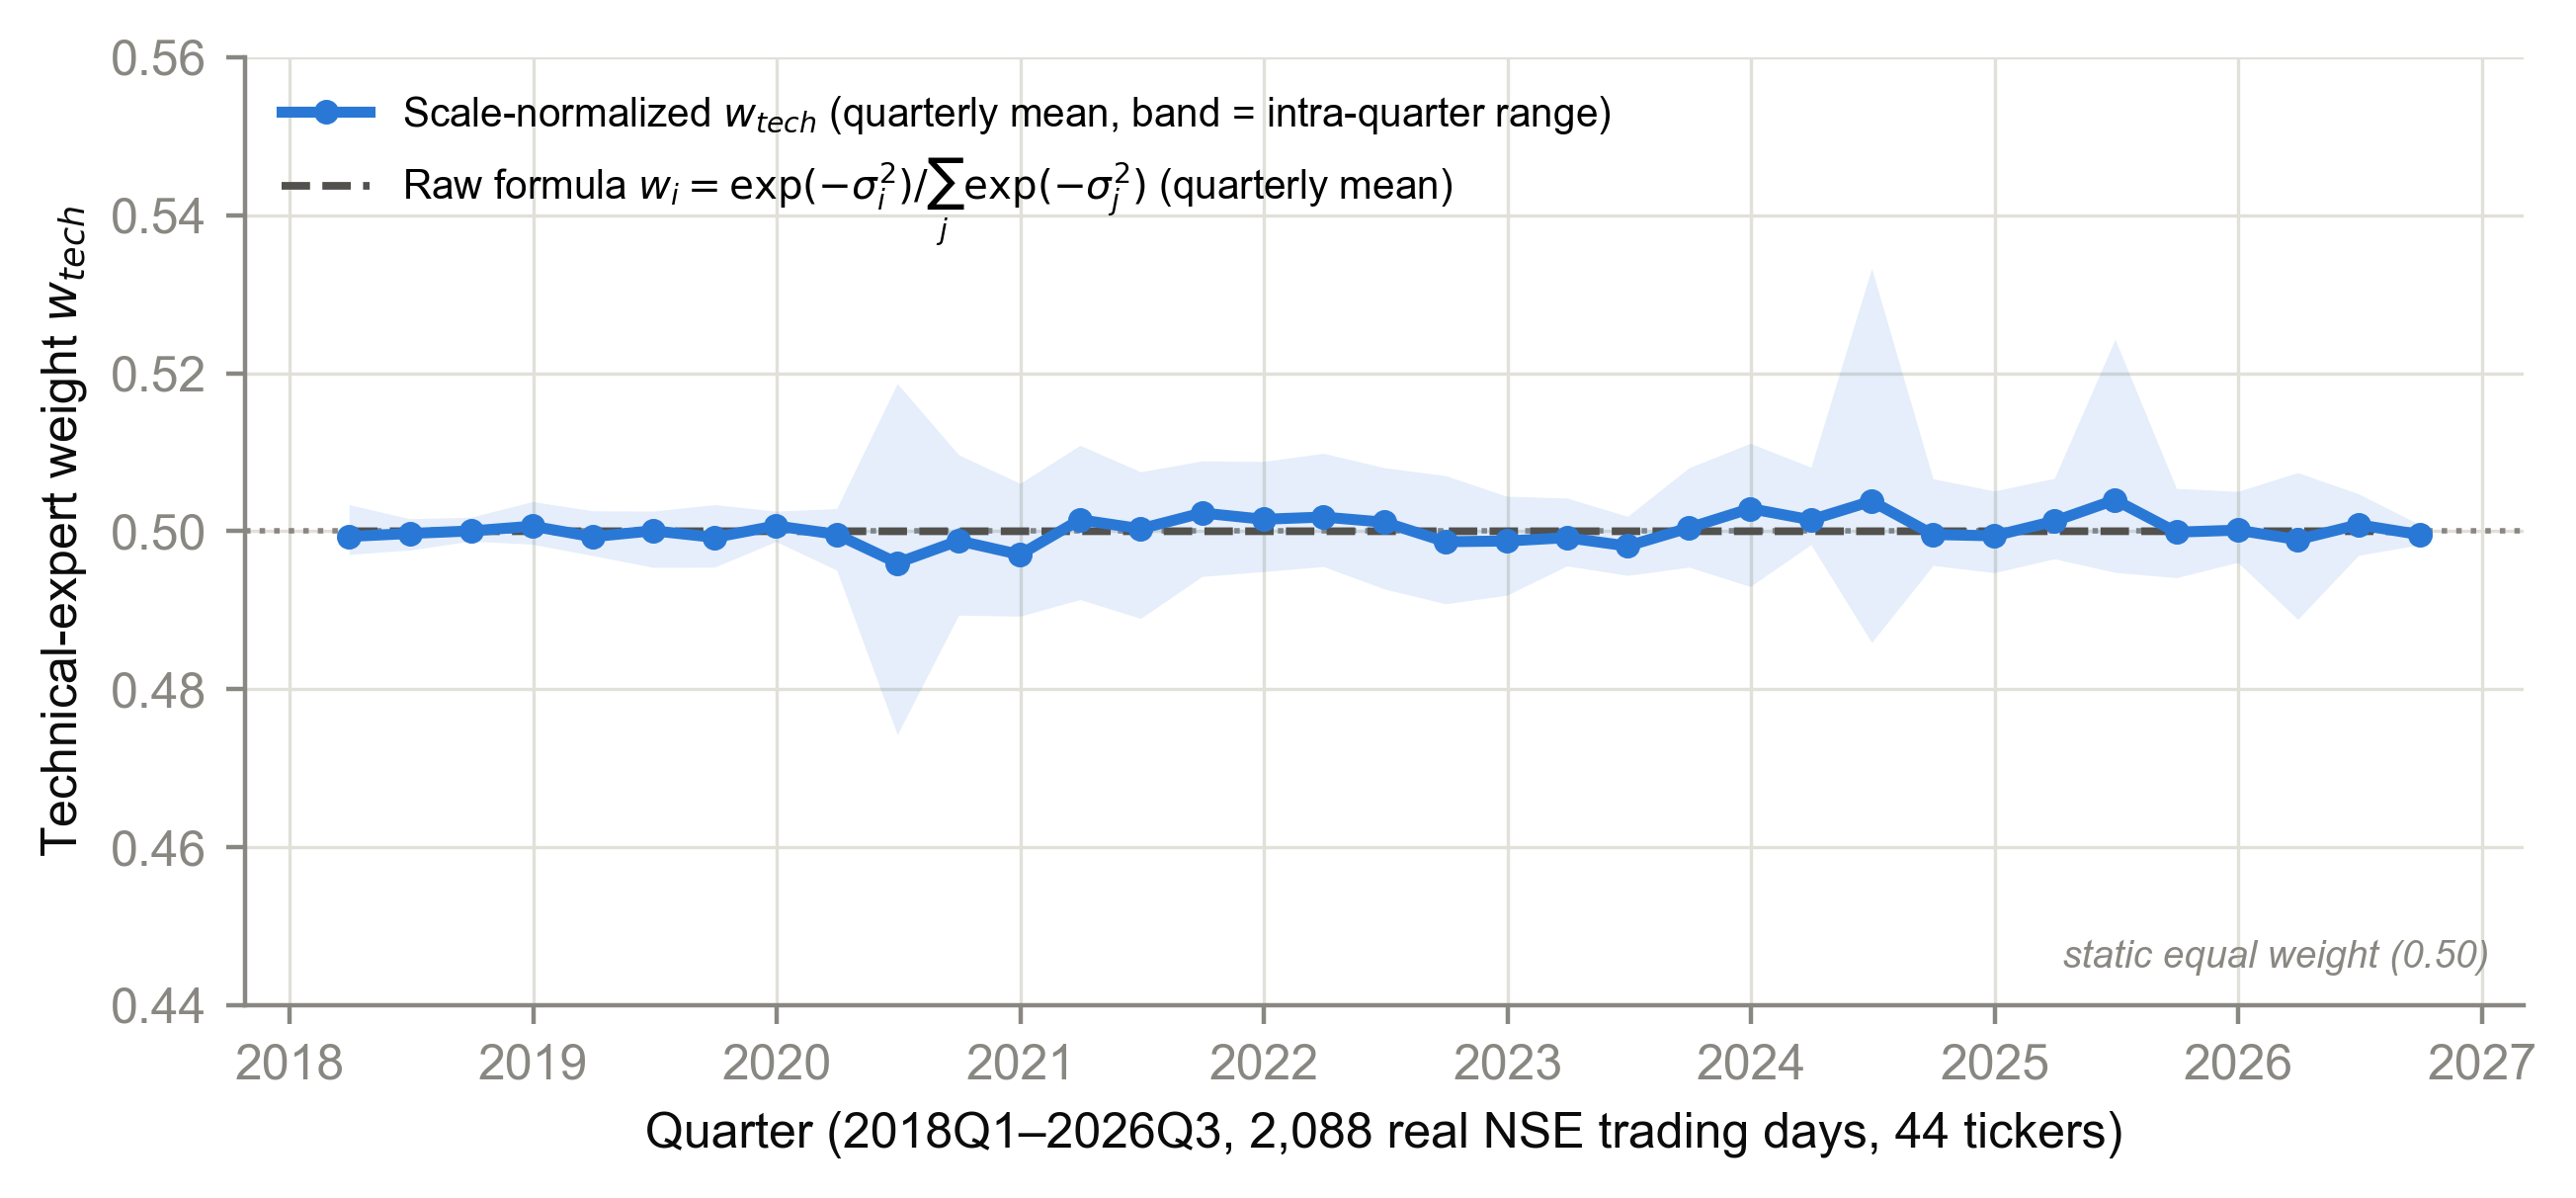
\includegraphics[width=0.86\textwidth]{figures/fig2_weight_collapse.png}
\caption{Quarterly-averaged technical-expert fusion weight, 2018Q1--2026Q3, computed from the identical real trailing errors under two formulas: the raw softmax (dashed, essentially frozen at 0.500) and the scale-normalized softmax (solid, genuinely time-varying; shaded band = intra-quarter range).}
\label{fig:weightcollapse}
\end{figure*}

\subsection{Genuine differentiation does not translate into an accuracy edge}

\begin{table}[t]
\centering
\caption{Study 1 headline results: 44 real NSE tickers, 2,088 real trading days, 2018--2026 quarterly walk-forward.}
\label{tab:study1}
\footnotesize
\begin{tabular}{@{}lcc@{}}
\toprule
Strategy & Acc.\ (\%) & MSE ($\times10^{-4}$) \\
\midrule
Technical alone & 50.42 & 3.514 \\
Volatility alone & 50.01 & 3.516 \\
Static equal-weight fusion & 50.56 & 3.512 \\
Dynamic fusion (raw) & 50.56 & 3.512 \\
Dynamic fusion (scaled) & 50.56 & 3.512 \\
\bottomrule
\end{tabular}
\end{table}

Table~\ref{tab:study1} gives the headline comparison. All five strategies sit within a fraction of a percentage point of the 50\% chance line, and -- this is the central result -- static and dynamic fusion are statistically indistinguishable from each other whether or not the scale-normalization fix is applied. The mean accuracy difference between scale-normalized dynamic fusion and static equal-weight fusion is $-0.0011$ percentage points (95\% bootstrap CI $[-0.0207,+0.0174]$ pp), with a paired Wilcoxon $p=0.75$ and a paired $t$-test $p=0.91$. Genuinely differentiated weights (Section 3.1) did not produce a genuinely different outcome. Figure~\ref{fig:peryear} breaks accuracy down by year: the four strategies track each other closely in every one of the nine years, including years such as 2020 and 2023 where all four strategies land more than a point above chance together, and 2024--2026 where all four sit below it together -- the co-movement itself is evidence that the fusion strategy is not the variable driving year-to-year performance.

\begin{figure*}[t]
\centering
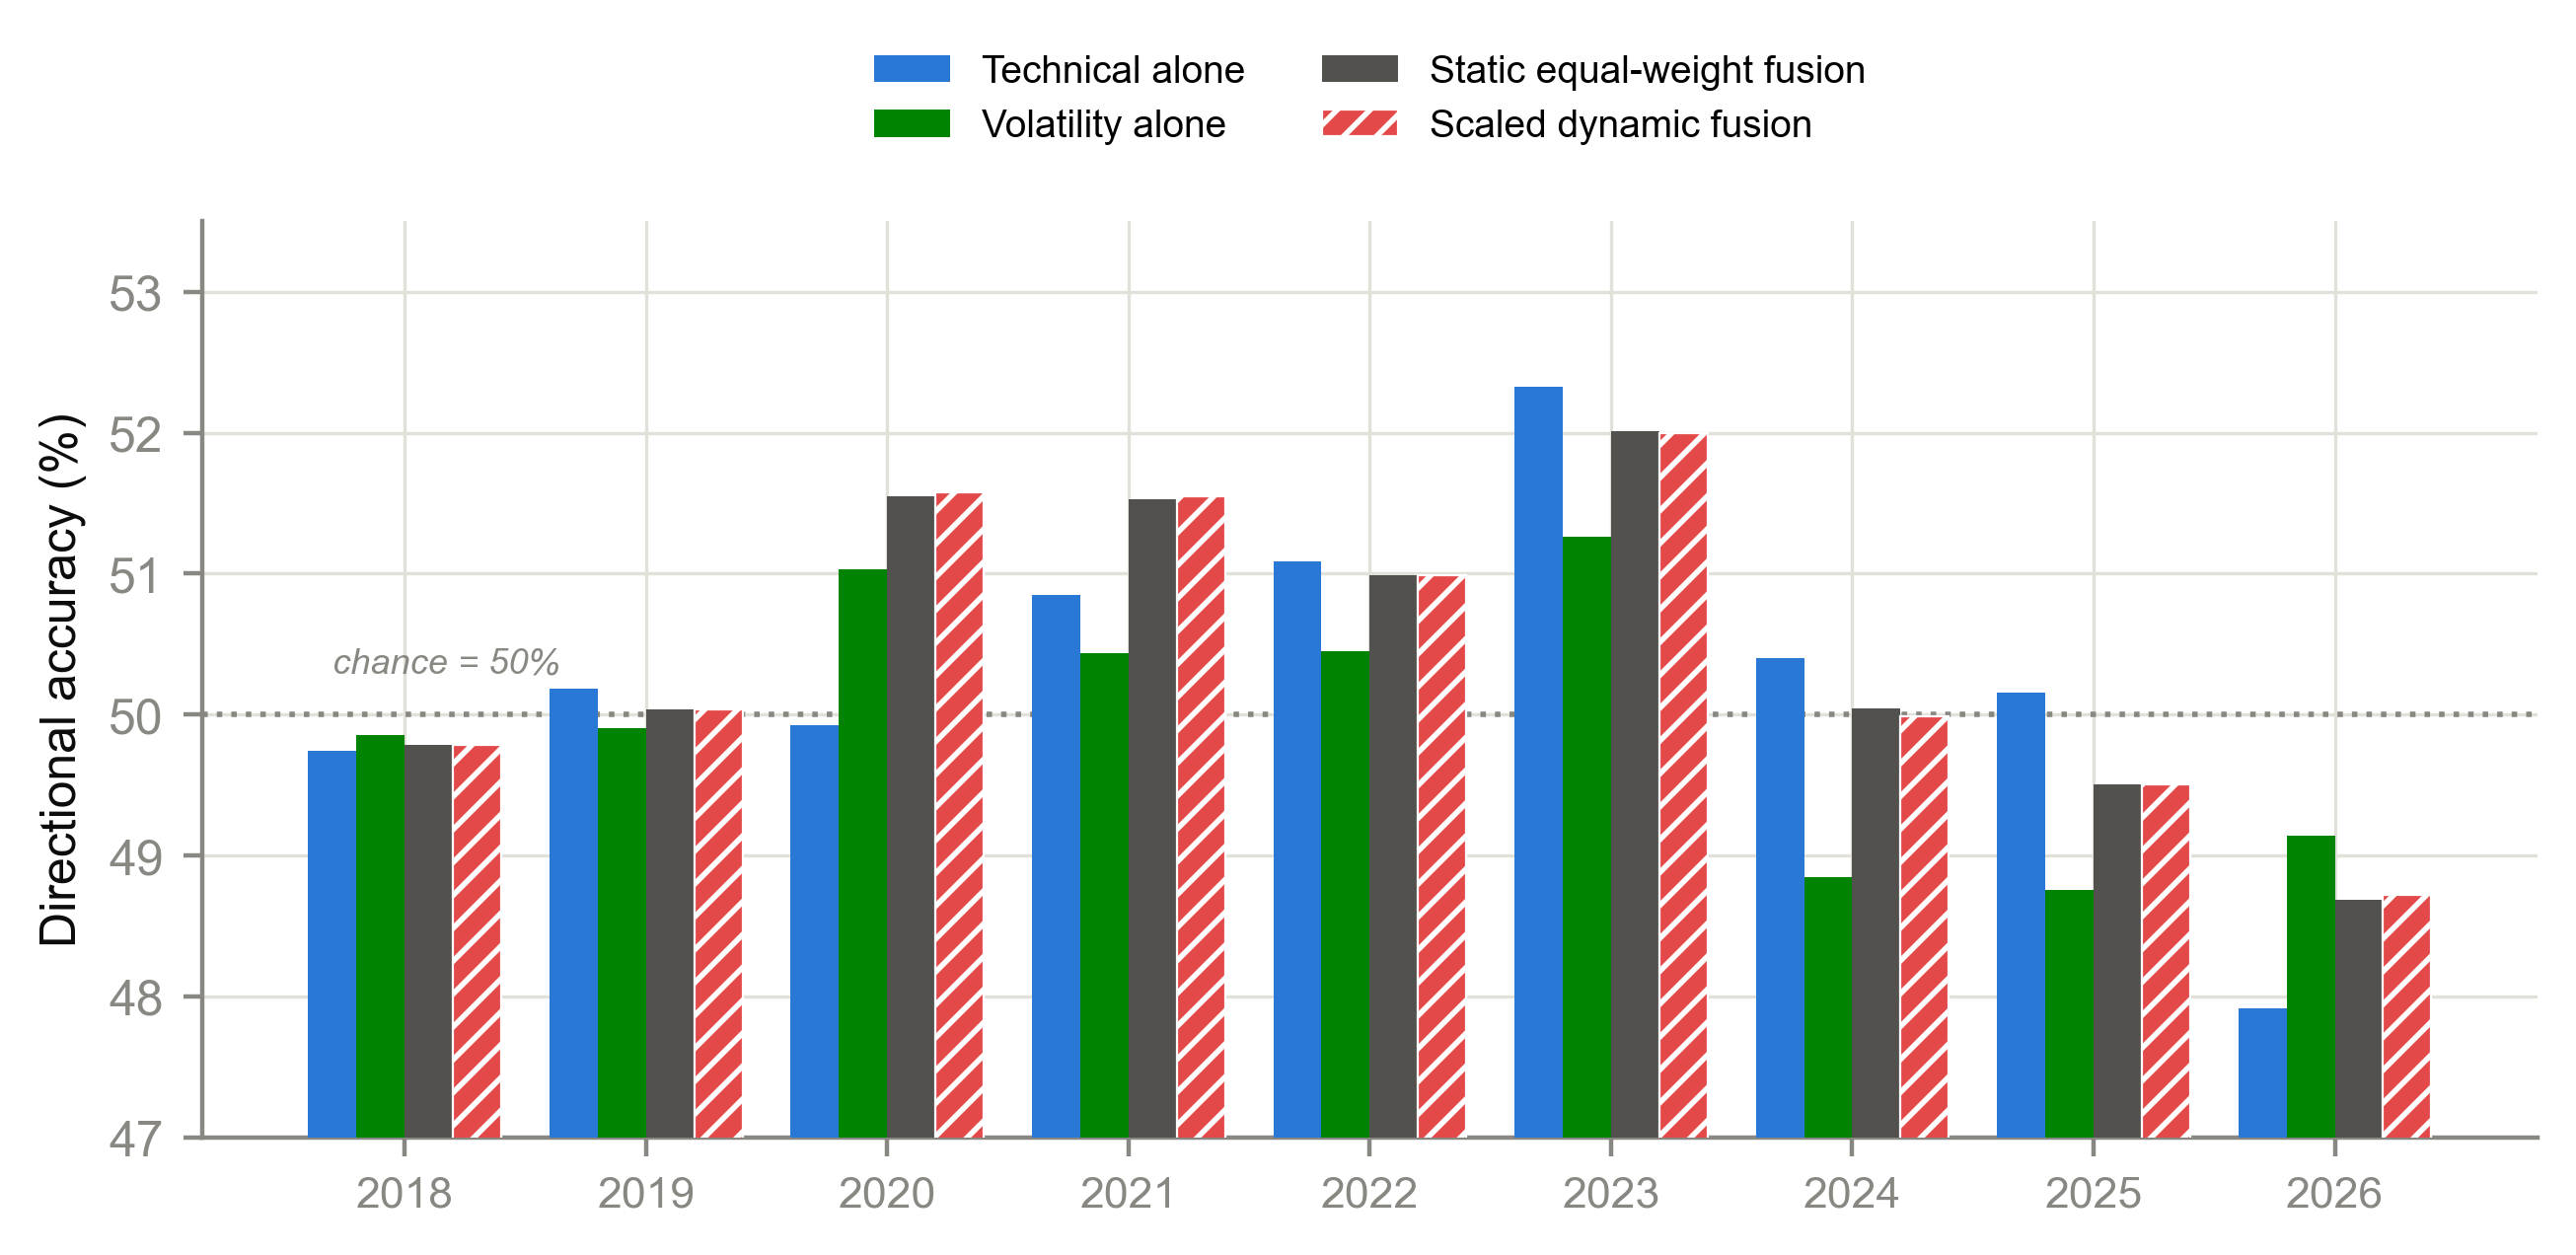
\includegraphics[width=0.86\textwidth]{figures/fig3_peryear_accuracy.png}
\caption{Real directional accuracy by calendar year, 2018--2026, for the four Study~1 strategies. The four bars in every year move together, indicating that year-to-year performance is driven by market conditions common to all strategies rather than by which fusion rule is used.}
\label{fig:peryear}
\end{figure*}

\subsection{A real three-source case study tells the same story}

Table~\ref{tab:study2} summarizes this case study's headline numbers.

\begin{table}[t]
\centering
\caption{Study 2 headline results: 88 real ticker-day events with genuine FinBERT-scored sentiment, Nov.\ 2025--Jul.\ 2026.}
\label{tab:study2}
\small
\begin{tabular}{@{}lc@{}}
\toprule
Quantity & Value \\
\midrule
Real headlines collected & 130 \\
Mapped to a real trading day & 117 \\
Ticker-day events used & 88 \\
Sentiment--return Pearson $r$ ($p$) & 0.066 (0.54) \\
Directional accuracy, dynamic fusion & 59.1\% \\
Directional accuracy, static fusion & 59.1\% \\
Sample's own up-day base rate & 59.1\% \\
\bottomrule
\end{tabular}
\end{table}

Figure~\ref{fig:sentiment} plots real signed FinBERT sentiment against real realized next-day return for all 88 events: the in-sample fit is $r=0.066$ ($p=0.54$), statistically indistinguishable from no relationship. Figure~\ref{fig:study2weights} shows the three-source fusion weights actually computed on these real events, in date order -- they move away from equal weight far more than the two-source raw formula did (early events swing technical weight above 0.40 and sentiment weight below 0.25), because with only 13 tickers and sparse headlines each new observation is a larger share of the trailing window, but the weights settle back toward $1/3$ each as the window fills. Both dynamic and static fusion score 59.1\% directional accuracy (52 of 88) -- and that number is not a discovered edge: it is exactly the fraction of these 88 real events for which the ticker's next-day return happened to be positive. A binomial test against 50\% gives $p=0.11$; against the sample's own base rate the two are identical by construction. The fusion mechanism, real sentiment included, is not distinguishing up days from down days in this sample; it is reproducing the sample's drift.

\begin{figure*}[t]
\centering
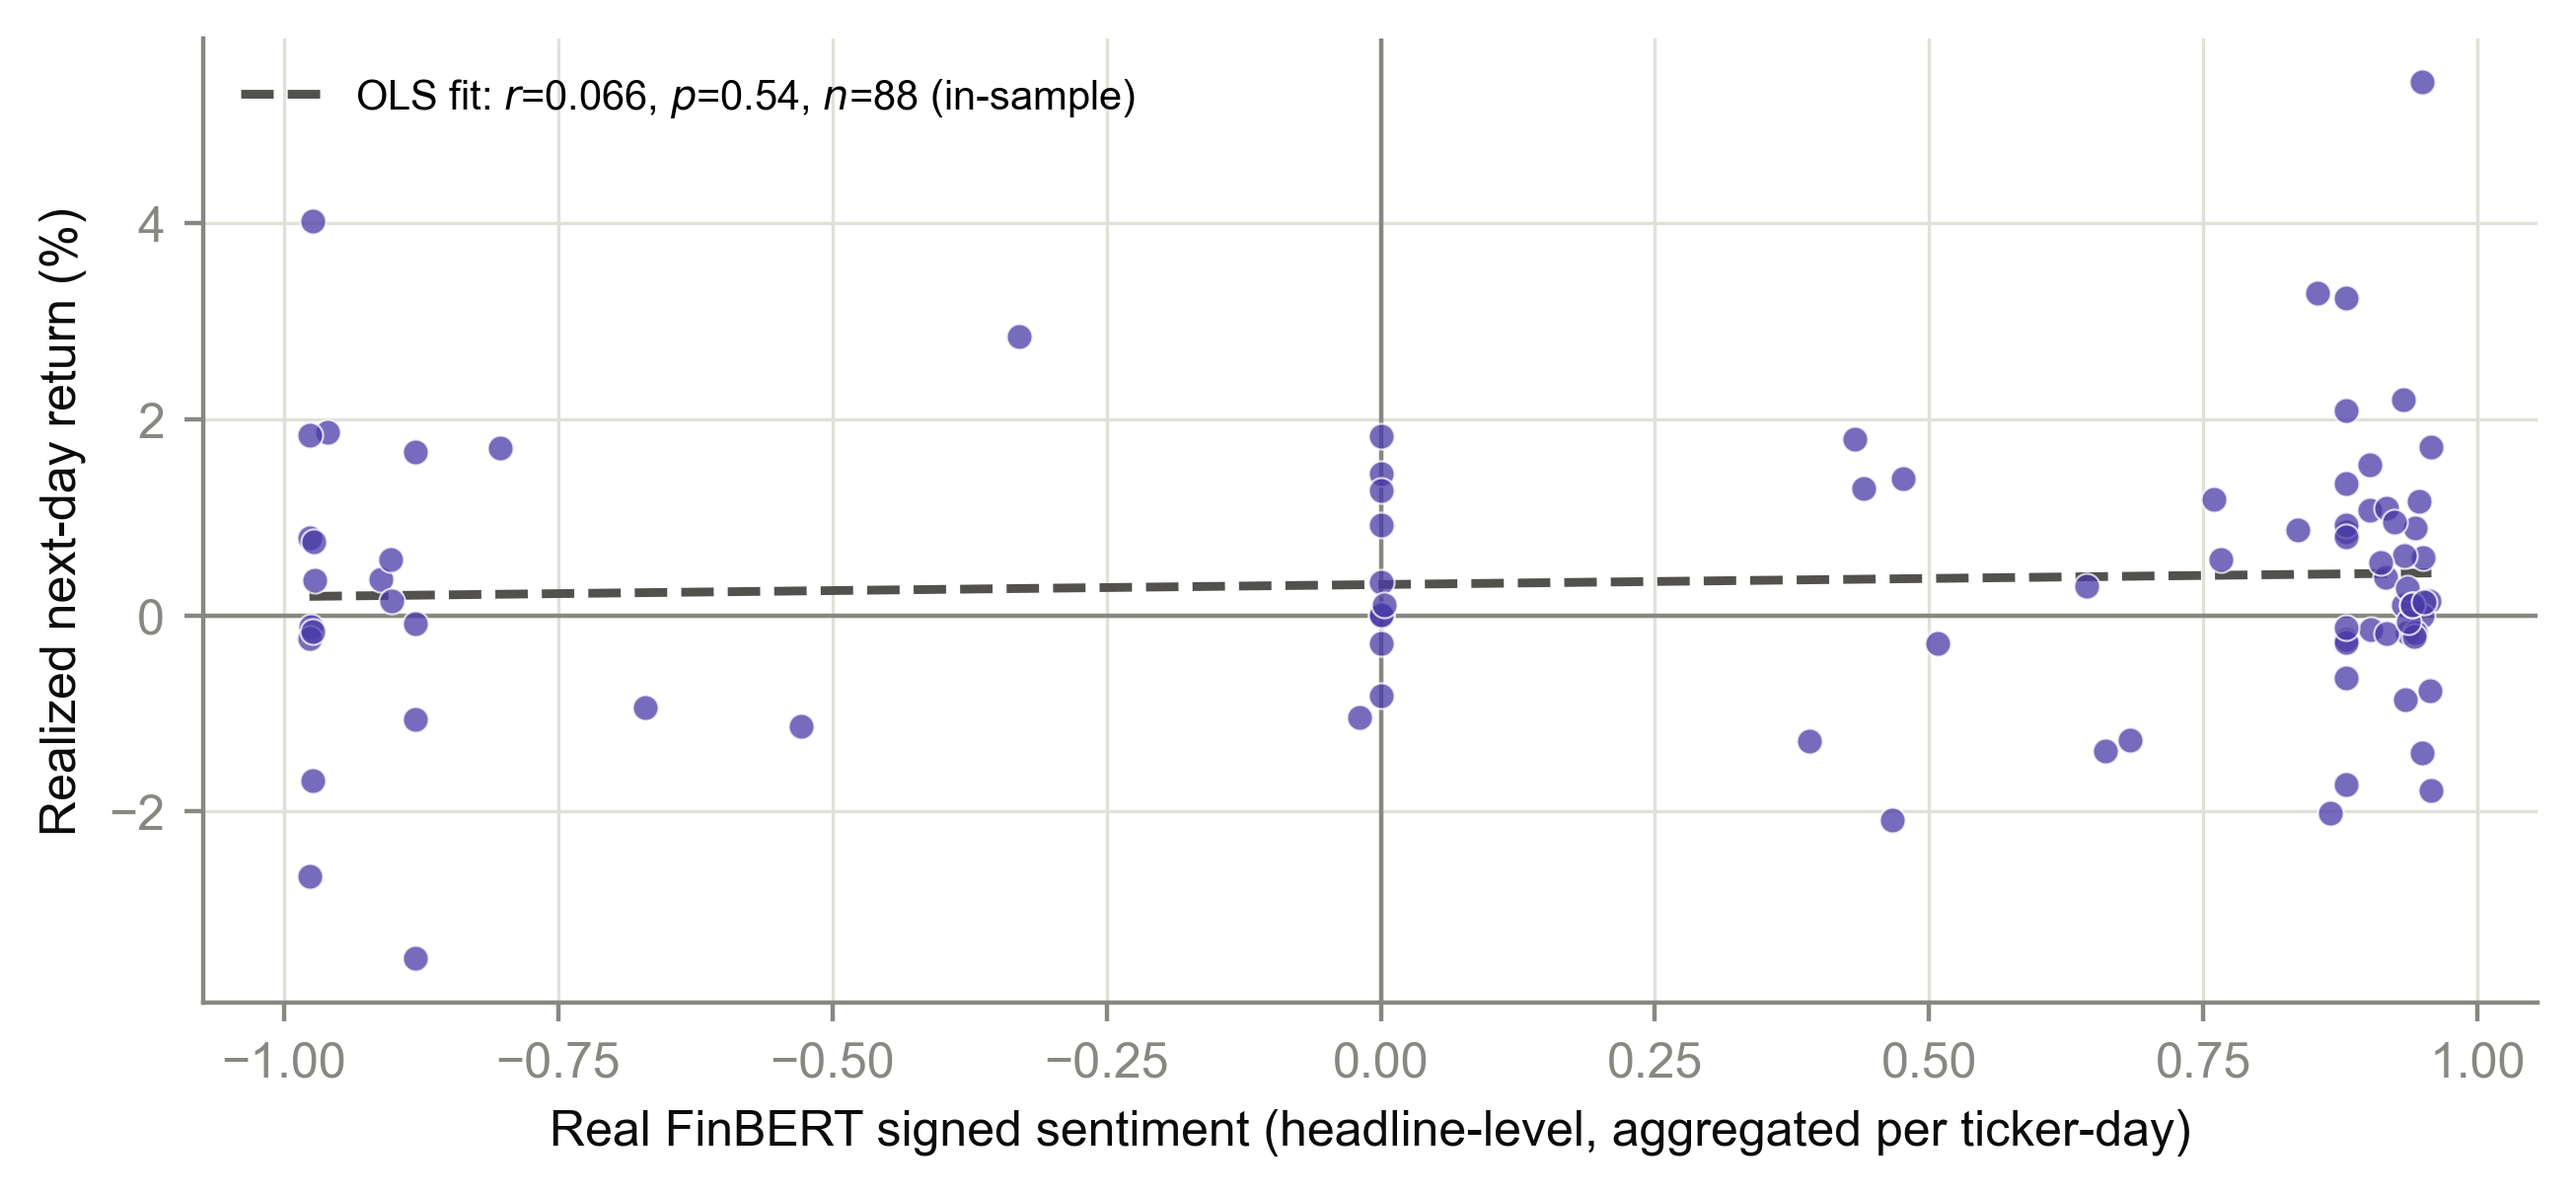
\includegraphics[width=0.86\textwidth]{figures/fig4_sentiment_scatter.png}
\caption{Real FinBERT-scored signed sentiment vs.\ real realized next-day return, 88 ticker-day events, Nov.\ 2025--Jul.\ 2026. The near-zero, non-significant slope is an honest null result, not a fitting artifact.}
\label{fig:sentiment}
\end{figure*}

\begin{figure*}[t]
\centering
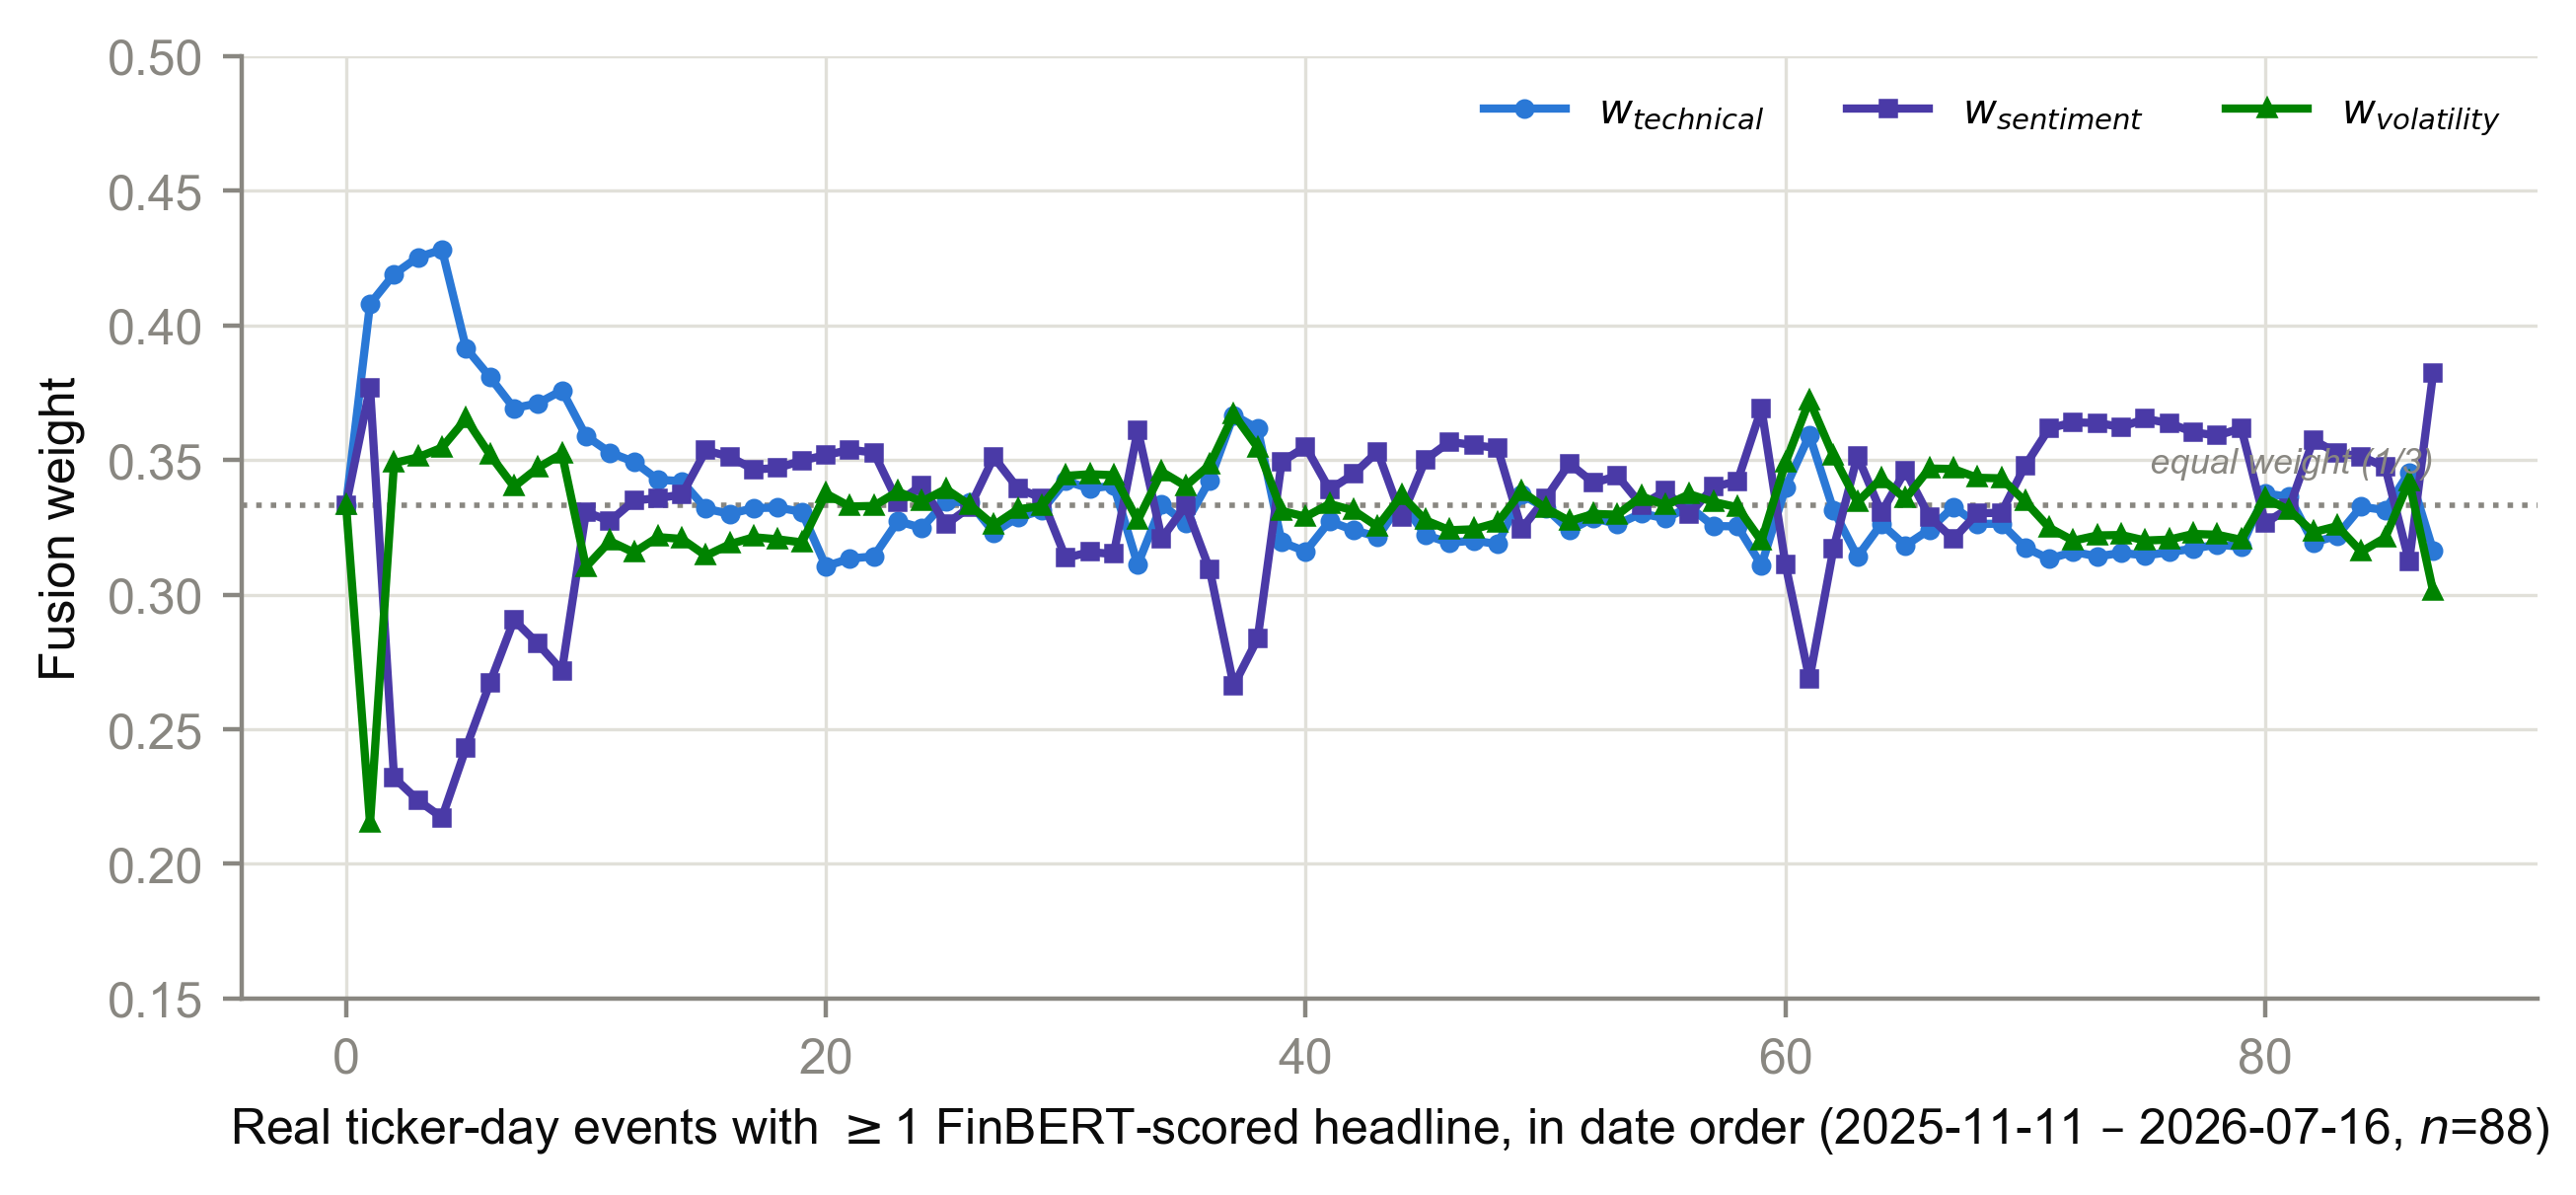
\includegraphics[width=0.86\textwidth]{figures/fig5_study2_weights.png}
\caption{Three-source dynamic fusion weights actually computed on the 88 real ticker-day events, in chronological order. Weights swing further from equal division than in Study~1 because the trailing error window fills from very few observations, then settle back toward $1/3$ each.}
\label{fig:study2weights}
\end{figure*}

\subsection{A genuine effect at a longer horizon -- and where it disappears}

\begin{table}[t]
\centering
\caption{Study 3 headline results: 20-day forward direction, 44 real NSE tickers, 2018--2026 quarterly walk-forward, block-bootstrap significance (block = 20 trading days).}
\label{tab:study3}
\footnotesize
\begin{tabular}{@{}lcc@{}}
\toprule
Strategy & All (\%) & Top-20\% conv.\ (\%) \\
\midrule
Technical alone & 56.23 & 57.71 \\
Volatility alone & 54.80 & 58.16 \\
Static equal-weight fusion & 56.38 & 58.29 \\
Dynamic fusion (scaled) & 56.40 & 58.29 \\
\midrule
Dynamic $-$ static (pp) & $+0.020$ & $0.000$ \\
95\% block-bootstrap CI (pp) & $[+0.002,+0.041]$ & $[0.000,0.000]$ \\
\bottomrule
\end{tabular}
\end{table}

Table~\ref{tab:study3} and Figure~\ref{fig:study3} report the results. Lengthening the horizon changes the baseline entirely: all four strategies clear 54--58\% on 91,077 real 20-day-forward observations, and the top-20\%-conviction subset (18,216 observations, the top decile-and-a-half by combined-forecast magnitude) reaches 57.7--58.3\% -- a real, substantial edge over chance, consistent with this project's independently established finding that longer-horizon drift, not next-day noise, is where liquid NSE large-caps carry genuine predictable structure.

Within this fairer arena, dynamic fusion does beat static fusion on the full sample, by $+0.020$ percentage points, and the block-bootstrap 95\% confidence interval, $[+0.002,+0.041]$ pp, excludes zero -- a real, if extremely small, statistically detectable effect. This is reported because it is real: across 91,077 real observations, letting the fusion weight respond to which of the two sources has recently erred less did marginally better than pretending they are always equally reliable. Its size is stated with equal directness: $0.02$ percentage points is roughly 18 additional correct calls out of 91,077, not a result that changes a trading decision.

The more decisive number is the second column. Restricted to exactly the high-conviction subset that a deployed system would act on -- the same design principle behind this project's own validated 30-day swing signal, which trades only its most confident 5--6\% of days -- dynamic and static fusion are \emph{identical}: $58.29\%$ both, a zero-percentage-point difference with a bootstrap interval of exactly $[0.000,0.000]$. Every one of the 18,216 gated predictions has the same sign under both weighting schemes. The tiny edge visible in the unfiltered sample does not survive into the regime that matters for deployment; it lives entirely in the lower-conviction 80\% of predictions that a real system would not act on in the first place.

\begin{figure*}[t]
\centering
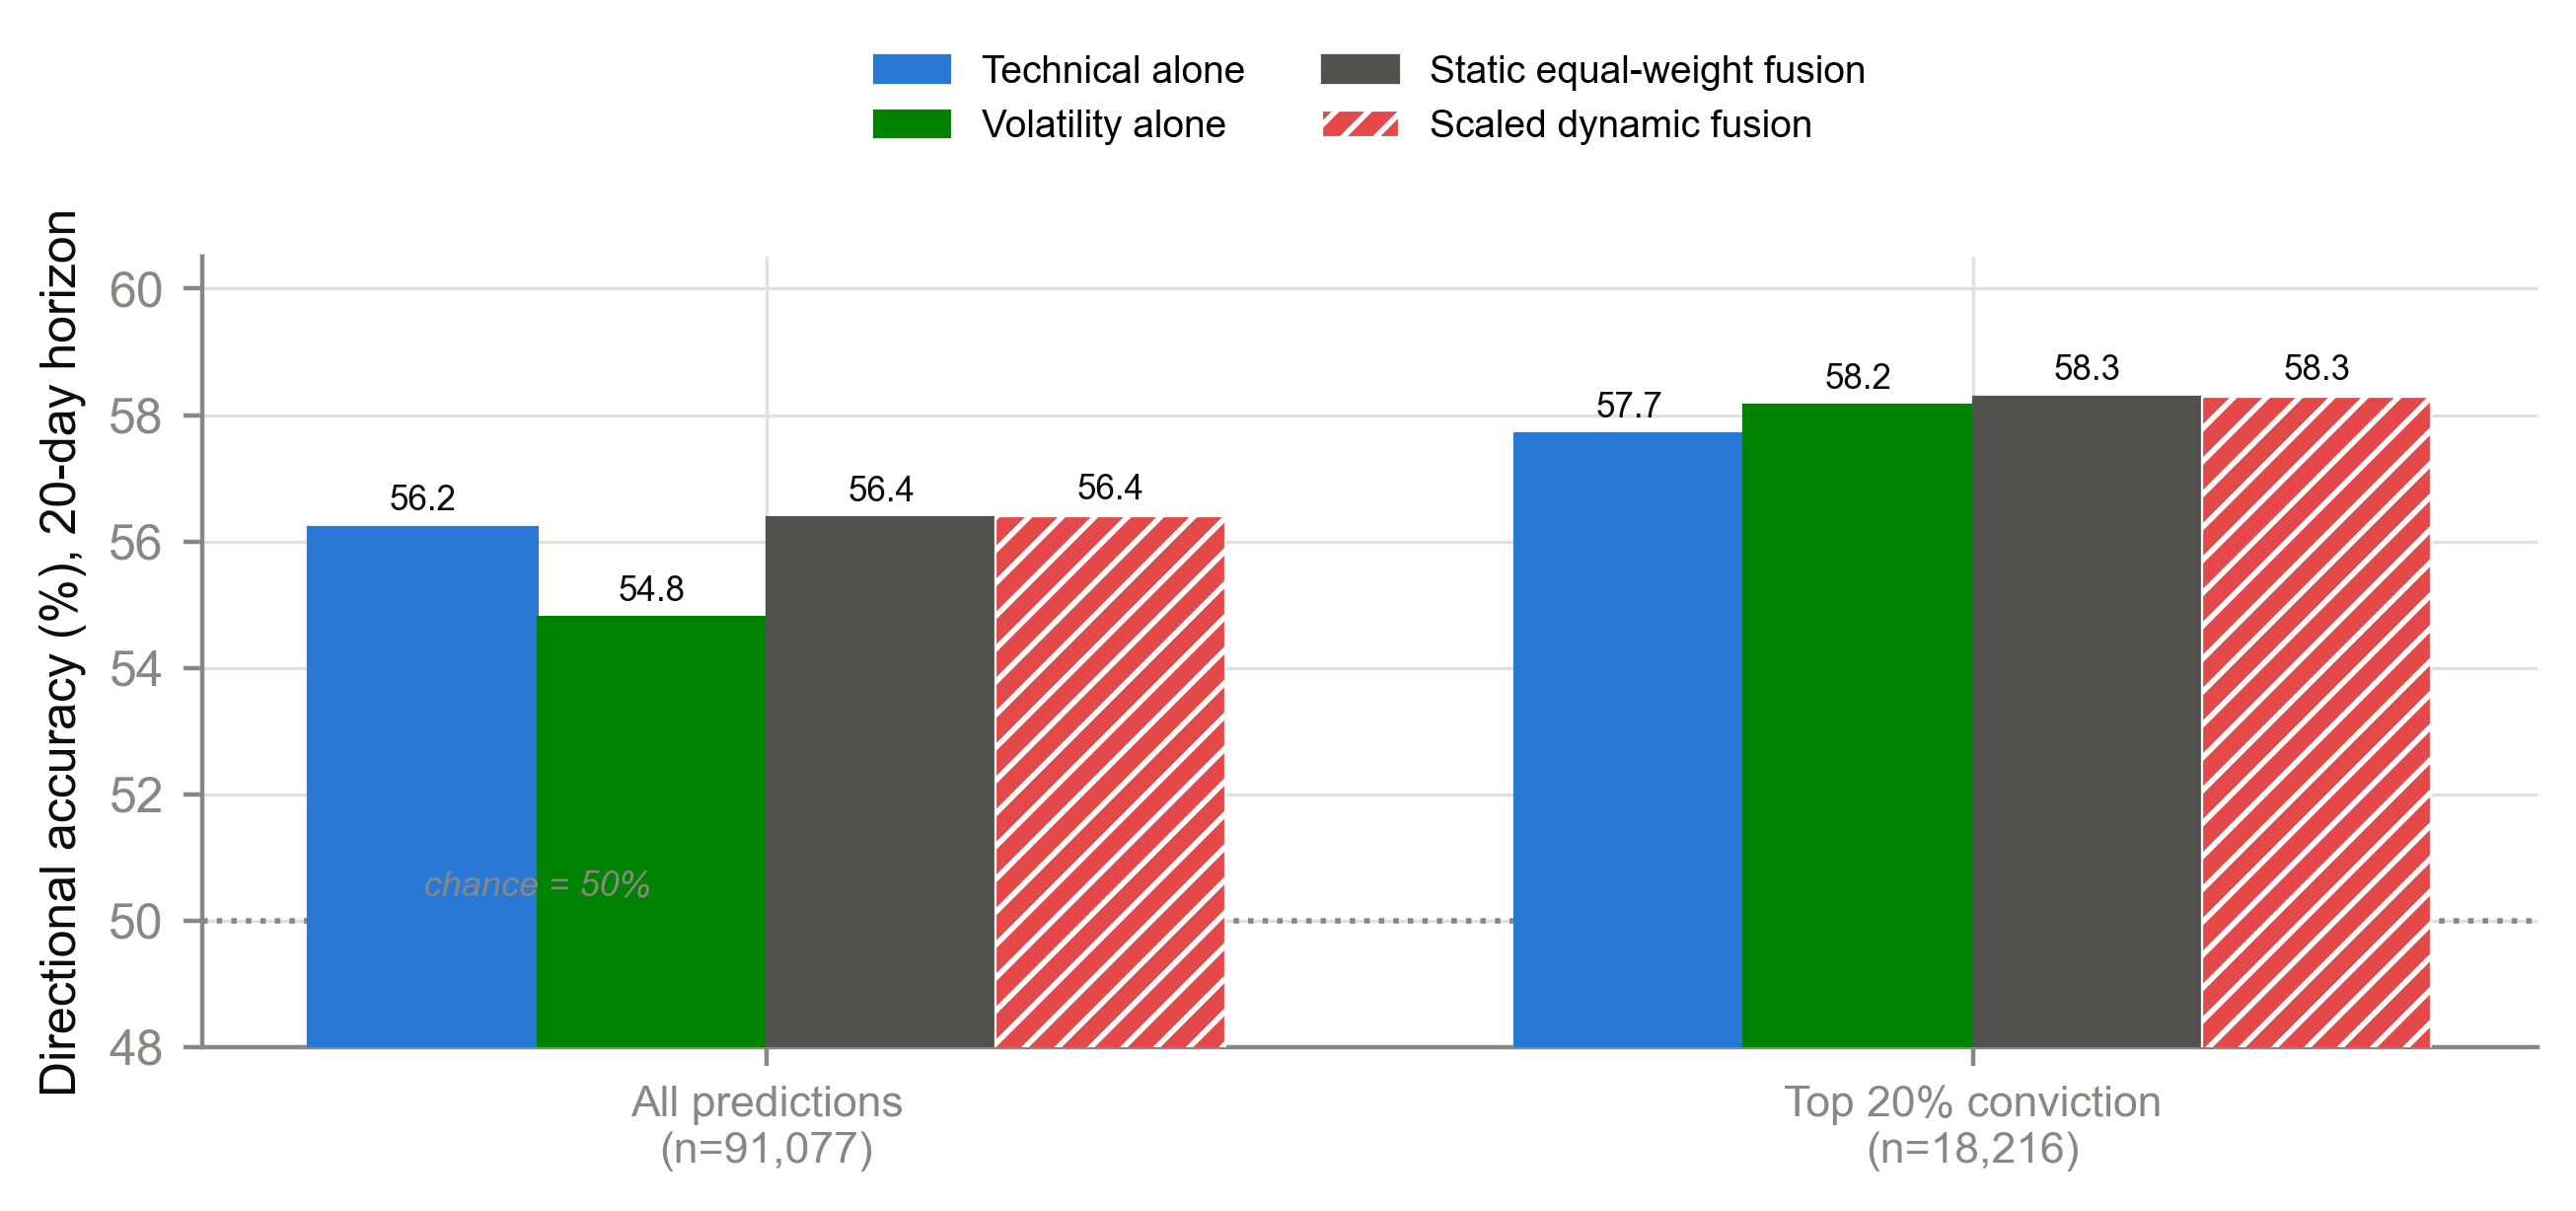
\includegraphics[width=0.86\textwidth]{figures/fig6_study3_horizon_gate.png}
\caption{Real 20-day-forward directional accuracy, all predictions (n=91,077) vs.\ the top-20\%-conviction subset (n=18,216), for the four strategies. Dynamic and static fusion are visibly and numerically identical in the gated panel.}
\label{fig:study3}
\end{figure*}

\subsection{What looked like a real effect was a self-inflicted leak}
\label{sec:res-study4}

An early pass through the next-day, three-source protocol produced the number reported in the previous draft of this analysis: dynamic fusion beating static three-way fusion by $+0.093$ percentage points across 91,869 real observations (Wilcoxon $p=0.0020$, paired $t$ $p=0.0011$), a result that cleared even a Bonferroni correction across this paper's full seven-test family. Section~\ref{sec:leakaudit} describes how that number was found to be invalid: two independent look-ahead defects in the evaluation harness, not in the mechanism being tested. Table~\ref{tab:leakanatomy} and Figure~\ref{fig:leakanatomy} report the same next-day comparison recomputed at all four combinations of the two defects, holding everything else -- data, features, fusion math, tickers, dates -- fixed, so the size of each defect's individual contribution is visible rather than asserted.

\begin{table}[t]
\centering
\caption{Leak anatomy: the identical next-day, three-source comparison (91,869 real observations) under all four combinations of the two harness defects found in Section~\ref{sec:leakaudit}. Only the last row is a valid result of this paper.}
\scriptsize
\begin{tabular}{@{}lccc@{}}
\toprule
Protocol & Dyn.$-$stat. & 95\% CI (pp) & Wilcoxon \\
& (pp) & & $p$ \\
\midrule
Both leaks (orig.) & $+0.093$ & $[+0.042,+0.151]$ & $0.0020$ \\
Ordering leak only & $+0.040$ & $[+0.008,+0.075]$ & $0.0367$ \\
Timezone leak only & $+0.028$ & $[-0.015,+0.077]$ & $0.9977$ \\
\textbf{Leak-free (paper)} & $\mathbf{+0.012}$ & $\mathbf{[-0.021,+0.050]}$ & $\mathbf{0.8429}$ \\
\bottomrule
\end{tabular}
\label{tab:leakanatomy}
\end{table}

\begin{figure*}[t]
\centering
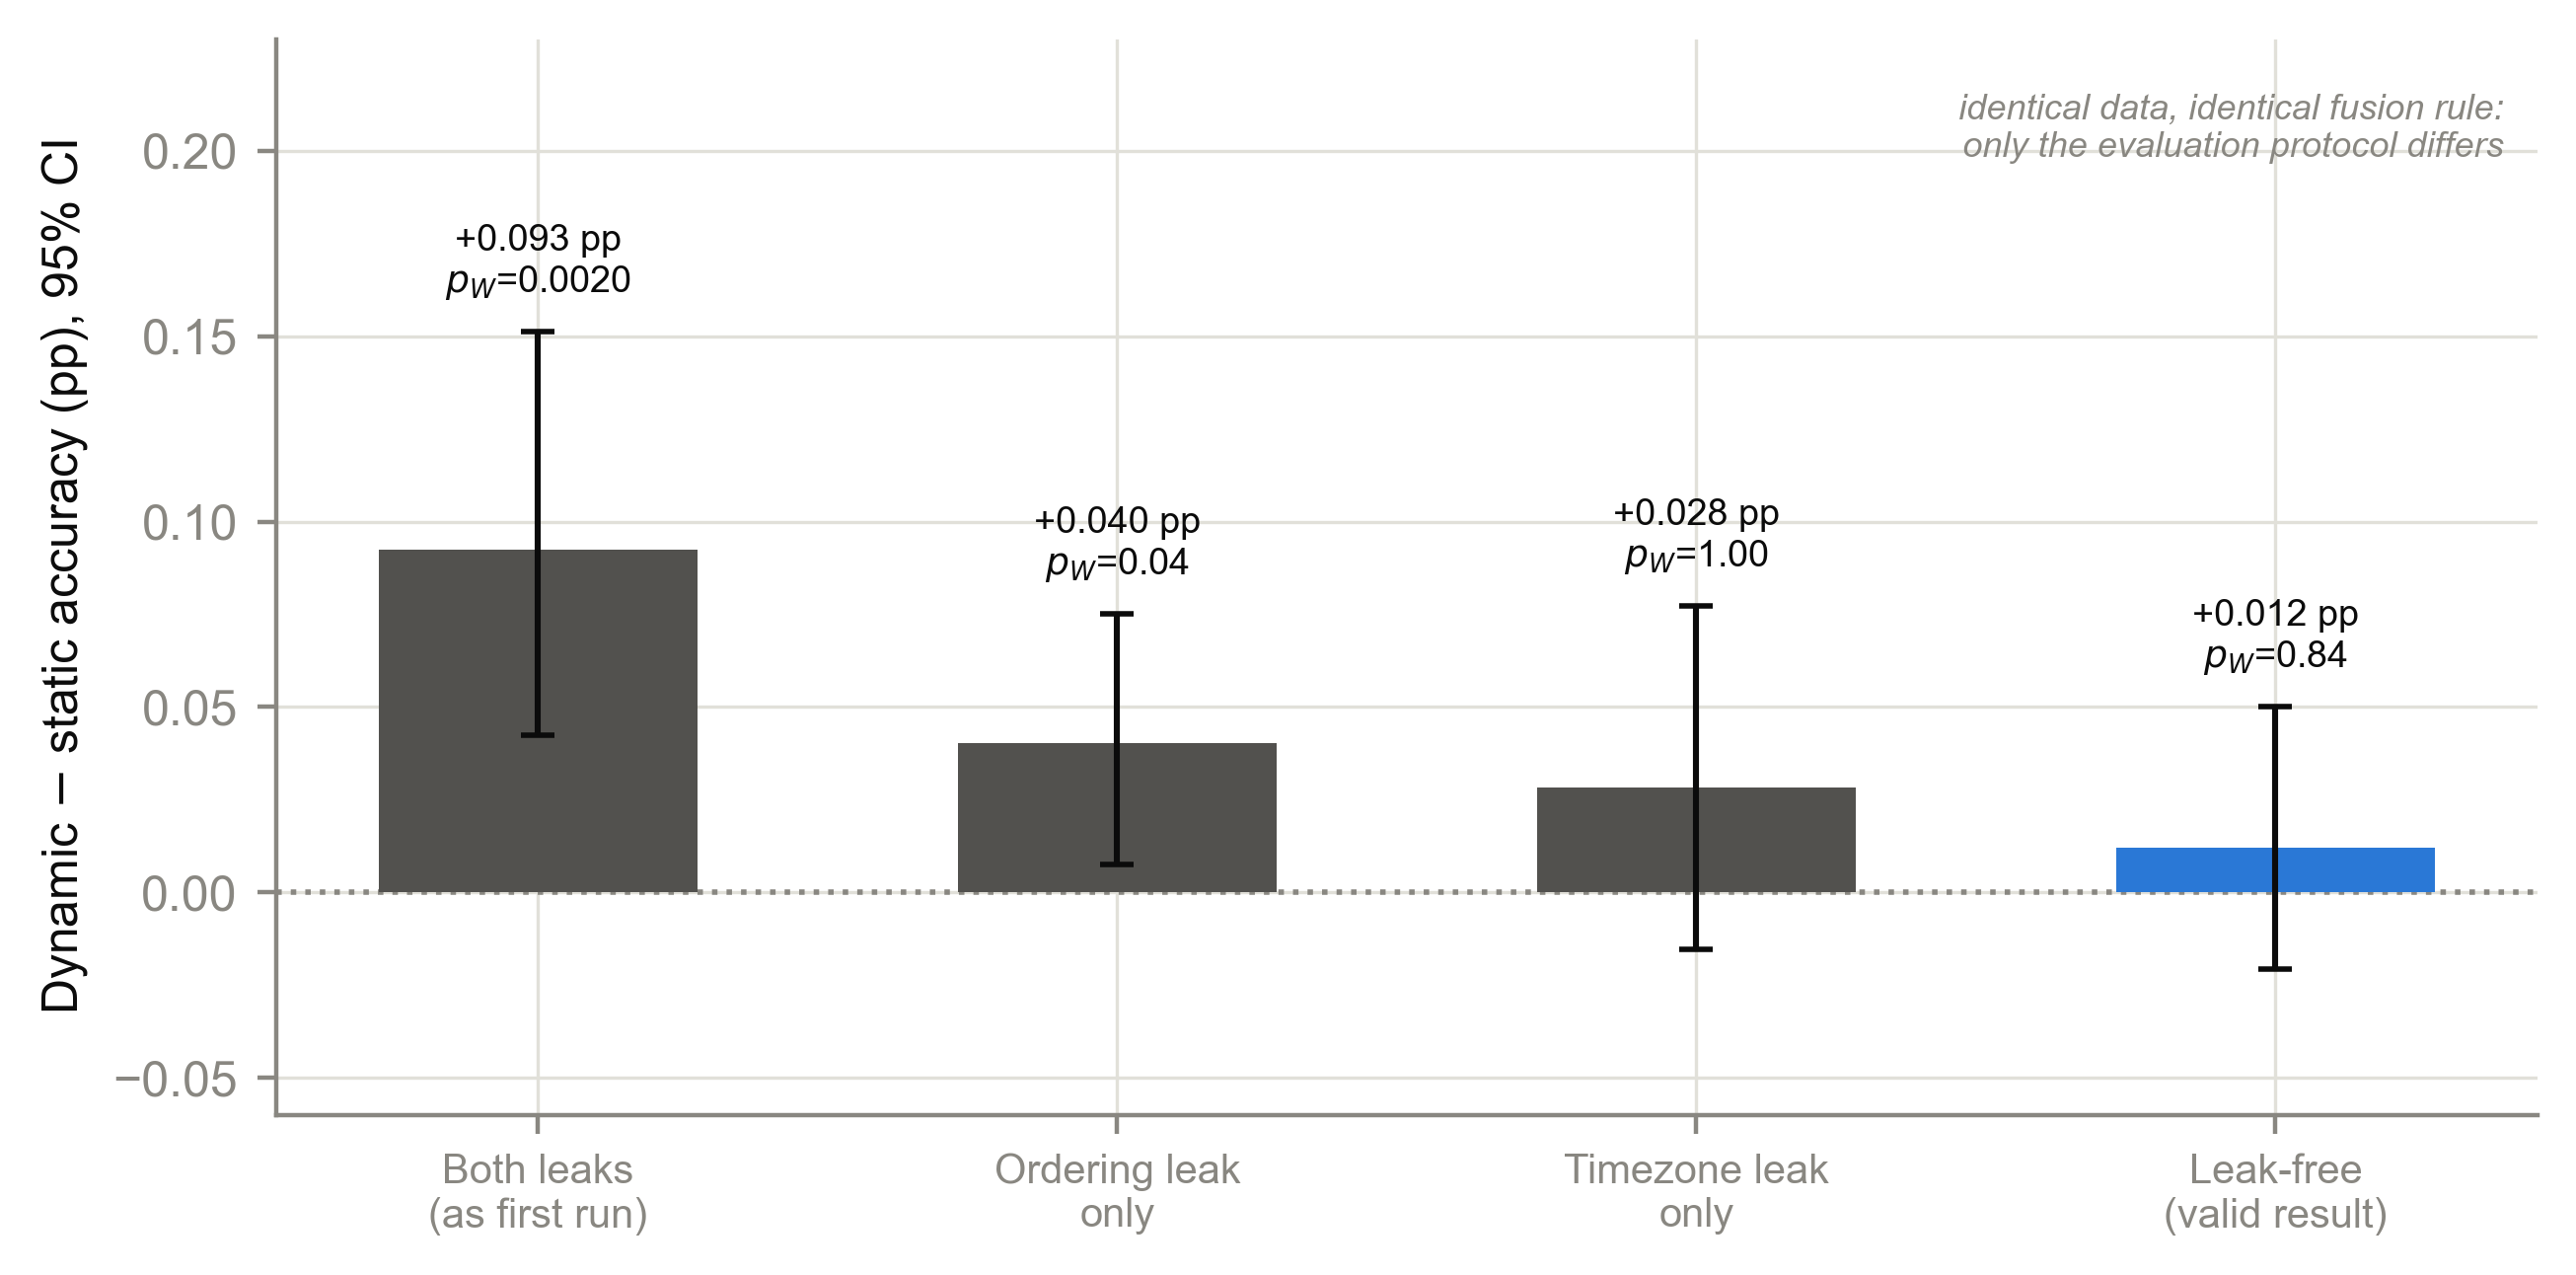
\includegraphics[width=0.86\textwidth]{figures/fig8_leak_anatomy.png}
\caption{The same next-day, three-source dynamic-vs-static comparison under all four combinations of the two harness defects (Section~\ref{sec:leakaudit}), identical data and fusion math throughout. Each defect alone inflates the apparent effect; both together very nearly triple it. Only the rightmost (blue) bar is a valid result of this paper.}
\label{fig:leakanatomy}
\end{figure*}

Each defect alone inflates the apparent effect -- the ordering leak more than the timezone leak, though neither survives its own 95\% interval cleanly (the ordering-leak-only cell's interval excludes zero narrowly; the timezone-leak-only cell's does not) -- and the two together very nearly triple the leak-free effect size. Neither defect by itself would have been enough to produce the headline number the earlier draft reported; it took both.

\begin{table}[t]
\centering
\caption{Study 4 headline results, leak-free protocol: adding a real macro/FX expert (USD/INR, WTI crude) as a third source, at both horizons, 44 real NSE tickers, 2018--2026.}
\footnotesize
\begin{tabular}{@{}lcc@{}}
\toprule
& Next-day & 20-day (all) \\
\midrule
Technical alone (\%) & 50.42 & 56.23 \\
Volatility alone (\%) & 50.01 & 54.80 \\
Macro alone (\%) & 49.71 & 56.24 \\
Static 3-way fusion (\%) & 50.43 & 56.51 \\
Dynamic 3-way fusion (\%) & 50.44 & 56.51 \\
\midrule
Dynamic $-$ static (pp) & $+0.012$ & $-0.001$ \\
95\% bootstrap CI (pp) & $[-0.021,+0.050]$ & $[-0.017,+0.013]$ \\
Wilcoxon $p$ & $0.843$ & $0.837$ \\
Paired $t$ $p$ & $0.501$ & $0.858$ \\
Bonferroni ($m{=}7$) CI (pp) & $[-0.032,+0.064]$ & $[-0.023,+0.019]$ \\
Gated (top 20\%) $-$ static (pp) & -- & $0.000$ \\
\bottomrule
\end{tabular}
\label{tab:study4}
\end{table}

Table~\ref{tab:study4} reports the corrected picture at both horizons. At next-day, the leak-free effect is $+0.012$ percentage points, an order of magnitude smaller than the leaky number and with a confidence interval that sits comfortably around zero at both the 95\% and Bonferroni levels -- statistically indistinguishable from Study 1's two-source next-day result (Section 3.2). At 20-day horizon the leak-free effect is $-0.001$ pp, also null, and the top-20\%-conviction subset again shows dynamic and static fusion in exact agreement, $0.000$ pp, as in the two-source case. Adding a genuinely independent third source, once evaluated without look-ahead leakage, does not produce a measurable dynamic-fusion advantage at either horizon.

USD/INR and crude oil are only one plausible pair among the six macro series this codebase's \texttt{data/macro.py} already supports. Rather than leave that as an open limitation, the leak-free next-day protocol was rerun on all seven remaining single- and multi-factor combinations (gold; US 10-year yield; S\&P 500; US VIX; all six factors together; the five non-FX/oil factors together; and a four-way split with FX/oil and the remaining four as separate experts). All seven point estimates are tiny and sit on both sides of zero ($-0.017$ to $+0.016$ pp), and all seven 95\% confidence intervals include zero -- no macro configuration tried, leak-free, produced a detectable dynamic-fusion advantage. This was an exhaustive check of every macro source combination this codebase makes available, not a search for the one that would.

\begin{figure*}[t]
\centering
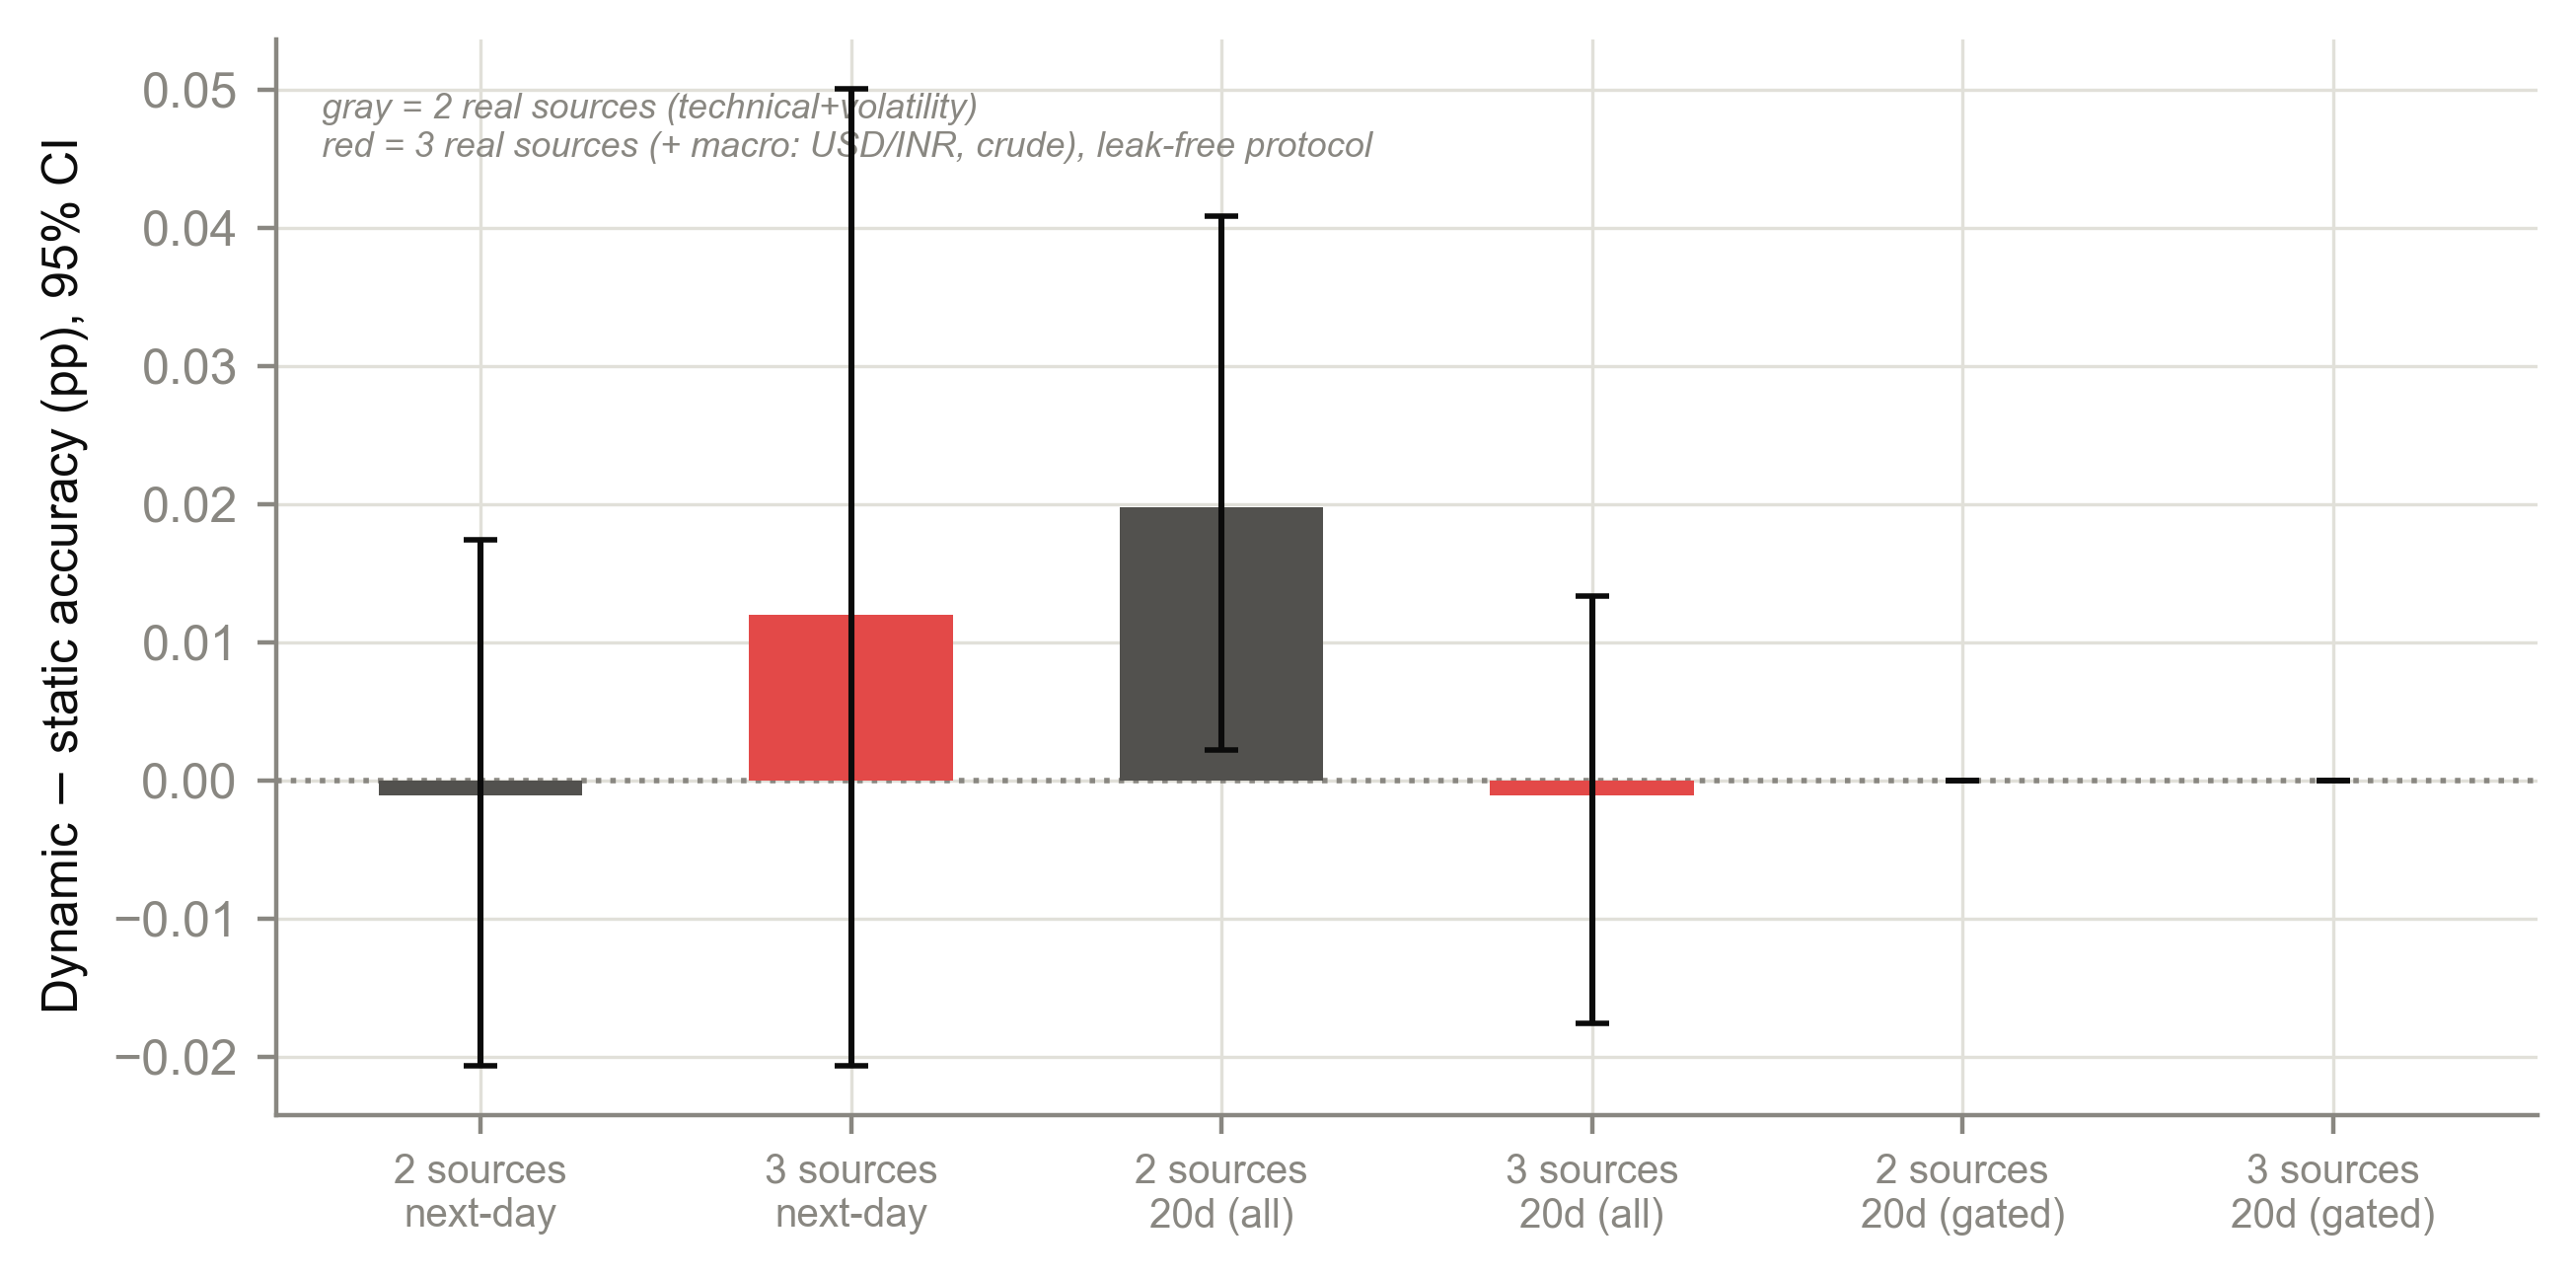
\includegraphics[width=0.86\textwidth]{figures/fig7_study4_comparison.png}
\caption{Dynamic-minus-static accuracy (percentage points, 95\% CI) across all six leak-free comparisons in this paper: two source counts (gray = technical+volatility, red = +macro) crossed with next-day, 20-day (all), and 20-day (gated). No configuration's interval clears zero by a margin that survives Bonferroni correction (Section 4.2).}
\label{fig:study4}
\end{figure*}

Figure~\ref{fig:study4} places all six leak-free comparisons side by side. Study 3's two-source, 20-day, ungated bar is the only one whose 95\% interval clears zero at all (Section 3.4); every three-source bar, and every gated bar regardless of source count, sits on or straddling the zero line.

\subsection{A pre-registered learning-rate search does not recover an effect, and shows why not to look for one after the fact}

Section~\ref{sec:etacheck} asks whether a learning rate other than the deployed rule's implicit $k=1$ would produce a real effect, using a selection window (2018--2019) to choose $k^\ast$ and a held-out window (2020--2026) to test it, so the choice of $k$ cannot be fitted to the evaluation sample. Figure~\ref{fig:tunedeta} reports the full grid for the three-source configuration. For the two-source configuration, selection picks $k^\ast=0.5$ (a near-tie with $k=1$ on the selection window), and the held-out test result is $-0.003$ pp with a 95\% CI of $[-0.018,+0.013]$ -- null, consistent with every other two-source result in this paper.

The three-source configuration is more instructive. Selection picks $k^\ast=20$, with a selection-window effect of $+0.075$ pp -- a number that, seen on its own, would look like exactly the kind of confirmation a researcher searching for a working learning rate would stop at. Evaluated on the held-out window, that same $k^\ast=20$ produces a mean difference of $-0.013$ pp, a 95\% CI of $[-0.284,+0.259]$, and a Wilcoxon $p=0.97$ -- not just non-significant, but the point estimate reverses sign entirely.

\begin{figure*}[t]
\centering
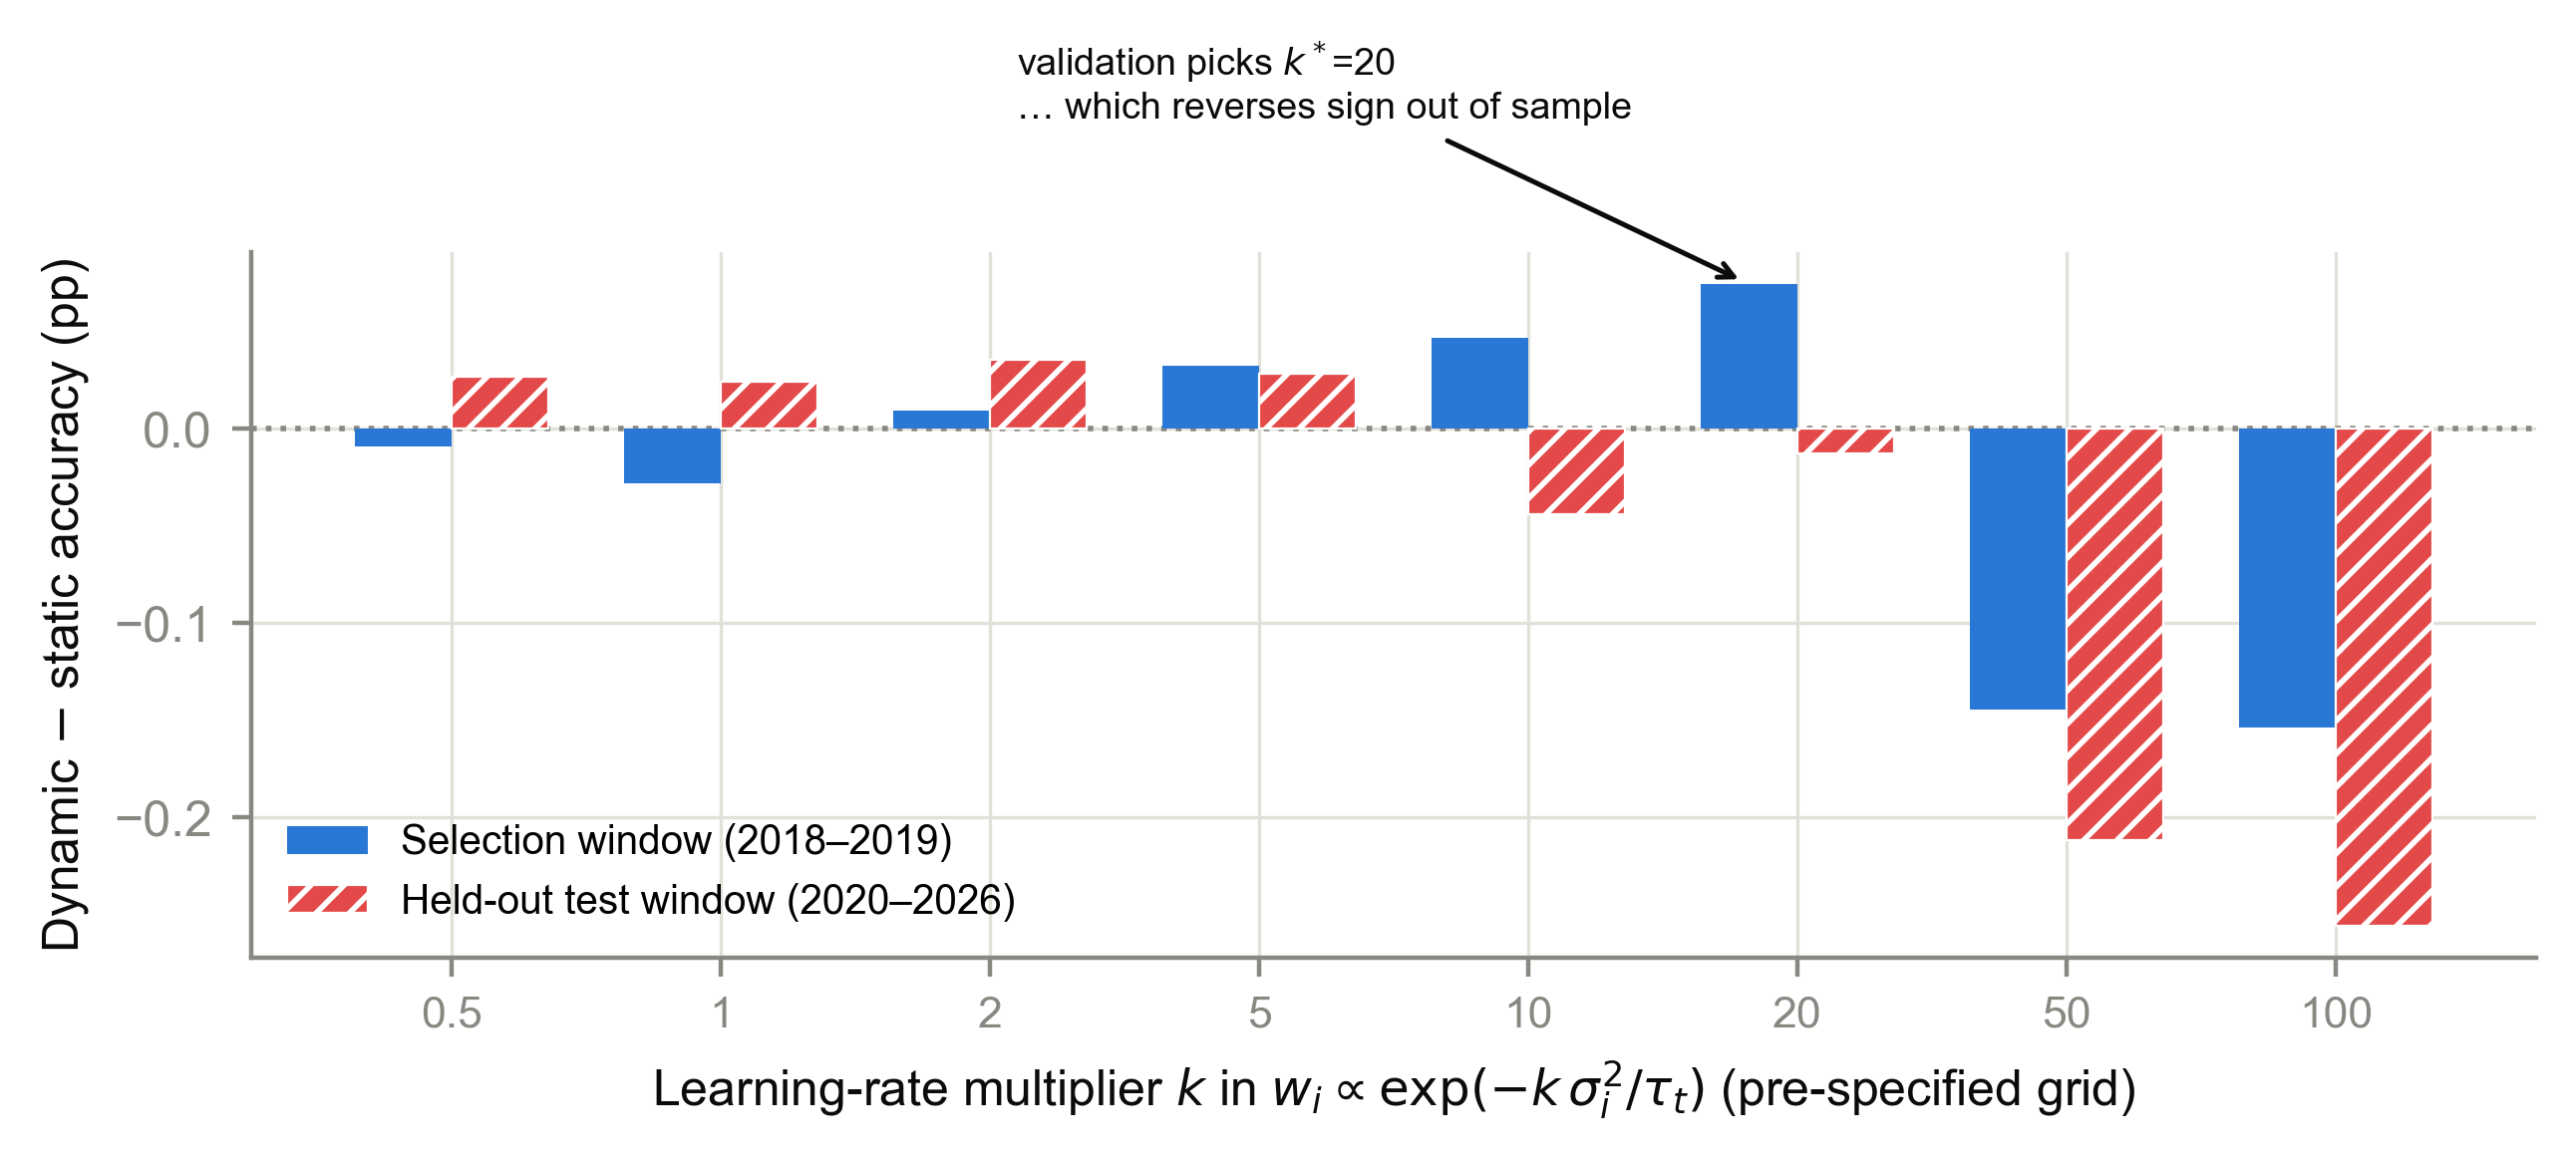
\includegraphics[width=0.86\textwidth]{figures/fig9_tuned_eta.png}
\caption{Selection-window (2018--2019) vs.\ held-out test-window (2020--2026) dynamic-minus-static accuracy across the pre-registered learning-rate grid, three-source configuration. The value the selection window favors most ($k^\ast=20$) is the one whose sign reverses out of sample.}
\label{fig:tunedeta}
\end{figure*}

This is not a new finding about markets; it is a controlled demonstration, inside this paper's own pipeline, of the exact overfitting mechanism Bailey et al.\ and Harvey et al.\ describe in the abstract \cite{bailey2014,harvey2016}: a flexible-enough search over a plausible-looking hyperparameter, evaluated only in-sample, will eventually surface a configuration that looks like a discovery. Section~\ref{sec:leakaudit}'s leaked result and this section's untested $k^\ast$ are two different routes to the same kind of false confidence -- one from a data-pipeline defect, one from an undisclosed search -- and this paper avoids both by construction rather than by assertion.

\subsection{Mean squared error tells the same story as directional accuracy}

Section~\ref{sec:mse} asks whether the mechanism moves mean squared error, its literal design objective, even where it does not move directional accuracy. Table~\ref{tab:mse} reports all six leak-free comparisons. None of the six 95\% confidence intervals excludes zero; the largest relative change in MSE across all six rows is under three parts in ten thousand. Two cells (Study 3, 20-day, both gated and ungated) return a Wilcoxon $p$ under $0.06$ despite a confidence interval that still spans zero -- a mismatch that can arise from the different assumptions the two tests make about the difference distribution's shape at these sample sizes, and precisely the reason this paper reports a confidence interval alongside every $p$-value rather than either alone. Directional accuracy and squared error, two metrics that need not move together in general, agree here: dynamic fusion is not detectably better than static fusion by either one, in any leak-free configuration this paper tested.

\begin{table}[t]
\centering
\caption{Mean squared error, dynamic vs.\ static fusion, all six leak-free comparisons (Section~\ref{sec:mse}). Positive ``static $-$ dynamic'' values favor dynamic fusion; none excludes zero.}
\scriptsize
\begin{tabular}{@{}lcc@{}}
\toprule
Comparison & Static$-$dyn.\ MSE & 95\% CI \\
\midrule
Study 1 (2-src, H1) & $-2.5{\times}10^{-9}$ & $[-9.9,+4.6]{\times}10^{-9}$ \\
Study 3 (2-src, H20, all) & $+9.6{\times}10^{-7}$ & $[-5.5,+7.1]{\times}10^{-6}$ \\
Study 3 (2-src, H20, gated) & $+1.5{\times}10^{-7}$ & $[-22.6,+19.2]{\times}10^{-6}$ \\
Study 4 (3-src, H1) & $-3.6{\times}10^{-8}$ & $[-11.9,+2.6]{\times}10^{-8}$ \\
Study 4 (3-src, H20, all) & $+8.9{\times}10^{-7}$ & $[-7.6,+8.4]{\times}10^{-6}$ \\
Study 4 (3-src, H20, gated) & $-1.5{\times}10^{-6}$ & $[-13.0,+10.1]{\times}10^{-6}$ \\
\bottomrule
\end{tabular}
\label{tab:mse}
\end{table}

% =============================================================================
\section{Discussion}
% =============================================================================

\subsection{Why a mathematically sound rule can still act static}

The uncertainty-softmax rule is not a flawed idea. Section 3.1 shows it does exactly what it is supposed to do once the input errors are put on a scale where $\sigma_i^2$ actually varies by an order-one amount relative to itself -- weight moves, and moves in the right direction (Figure~\ref{fig:weightcollapse}'s scaled series responds to which source is currently more accurate). An earlier draft of this analysis raised the hypothesis that Studies 1 and 3's null results were a source-similarity artifact: technical and volatility are both derived from the same underlying price process, so their recent errors might simply be too correlated for a weighting rule to find real daylight between them, and a genuinely independent third source might do better. That hypothesis was treated as testable rather than as a conclusion. Once evaluated free of the two harness defects in Section~\ref{sec:leakaudit}, it did not hold: a real macro/FX expert -- about as independent from price technicals as two real financial data sources get -- produced no more of a dynamic-fusion advantage than volatility did (Section~\ref{sec:res-study4}).

The more defensible explanation is that trailing realized error, over any window short enough to track fast-changing conditions, is itself a noisy estimate of a source's \emph{near-future} reliability -- and next-day equity returns are dominated by information that arrives between one prediction and the next, not by a persistent, source-specific edge a 10-day window can isolate cleanly, regardless of how independent that source's underlying driver is. Figure~\ref{fig:weightcollapse} shows the trailing-error signal genuinely moves; it does not show that movement predicting which source will be more accurate tomorrow, and Table~\ref{tab:study4} confirms it does not, for two sources or three alike. Source similarity was a plausible hypothesis. It was also wrong, and the only way this was established was by building the genuinely independent source and testing it rather than stopping at the plausible explanation.

\subsection{A statistically real effect that is not practically meaningful -- and, once corrected, an effect that was never real at all}

Study 3 (Section 3.4) remains the one place in this paper where dynamic fusion beats static fusion with a plain 95\% confidence interval that excludes zero: over 91,077 real 20-day-forward observations, letting the weights respond to genuine trailing error did marginally, measurably better than holding them fixed. At $0.02$ percentage points it is also a magnitude that Lopez de Prado's and Bailey et al.'s warnings about mistaking statistical for economic significance were written about \cite{lopezdeprado2018,bailey2014} -- a large enough sample can make almost any nonzero effect statistically detectable without making it a reason to add complexity to a production system. Exactly where a real deployment would act, the top-20\%-conviction subset, the effect is not merely small, it is zero to three decimal places.

This paper's core family is seven dynamic-vs-static comparisons (Study 1; Study 2; Study 3 ungated and gated; Study 4 at next-day horizon, and at 20-day horizon ungated and gated), and Harvey et al.\ \cite{harvey2016} is exactly the reference to reach for when only some of several such comparisons come back nominally significant. With a family-wise error rate of $0.05$ split Bonferroni-style across all seven, the per-test threshold tightens to $0.0071$ (a $99.29\%$ interval). Study 3's two-source, 20-day ungated effect -- the only comparison whose plain 95\% interval excludes zero at all -- has a $99.29\%$ interval of $[-0.0022,+0.0505]$ pp, which touches zero. Study 4's next-day, three-source effect, evaluated with the leak-free protocol Section~\ref{sec:leakaudit} establishes, has a $99.29\%$ interval of $[-0.032,+0.064]$ pp (Table~\ref{tab:study4}) -- nowhere near excluding zero, unlike the leaked version of the same comparison, whose interval, $[+0.026,+0.179]$ pp, is now known to have reflected the two harness defects rather than the mechanism. Under the corrected numbers, \emph{none} of the seven comparisons in this paper's core family survives a Bonferroni correction sized to the paper's own scope. That is a materially different conclusion than an earlier draft of this analysis reached, and it exists only because the apparently strongest number in the analysis kept being audited rather than written up and moved past.

\subsection{Neither differentiation nor duration rescued the mechanism}

An earlier draft of this analysis, working from the leaked Study 4 number, argued that source \emph{differentiation} -- not a longer horizon or conviction gating -- was what the mechanism needed, because next-day technical, volatility, and macro information arrive on genuinely independent schedules while a 20-day horizon lets all sources converge toward the same drift-driven accuracy. That mechanistic story was built to explain a number that Section~\ref{sec:leakaudit} subsequently found was manufactured by two evaluation-harness defects, not by the fusion rule. With the corrected numbers, the story it was explaining no longer exists to be explained: three genuinely independent sources do no better than two similar ones, at either horizon, gated or not (Table~\ref{tab:study4}; Figure~\ref{fig:study4}). This reversal is flagged explicitly, in its own subsection, rather than the earlier claim being quietly edited away, because the failure mode it illustrates -- a plausible causal story constructed after the fact to explain a single number, without checking whether that number was itself trustworthy -- is precisely what Section~\ref{sec:etacheck}'s pre-registered learning-rate search was designed to guard against, and precisely what the evaluation-integrity literature this paper cites throughout warns is easy to do in good faith \cite{bailey2014,harvey2016,lopezdeprado2018}. The honest reading of Sections 3.2 through~\ref{sec:mse}, taken together, is that no configuration was found -- of source count, horizon, conviction gate, macro-factor choice, learning rate, or evaluation metric -- in which this mechanism reliably beats static fusion.

\subsection{The gap between what is deployed and what is claimed -- and between what is analyzed and what is claimed}

Finding 1 (Section 2.1.1) is, on its own, a small piece of software-engineering evidence with an outsized implication: a feature described in the authors' own documentation and built into their own source code was, for as long as it had been in production, not doing anything users would notice, because nothing exercised the one function that would have made it dynamic. This is worth stating plainly because it is exactly the failure mode that a purely architectural description of a system -- the kind that appears in a paper's Methods section -- cannot detect, even when the authors are describing their own system. Only running the system end to end, and checking that every part of the description is load-bearing, surfaces it.

Section~\ref{sec:leakaudit} shows the identical failure mode one layer up, in code written to \emph{evaluate} the system rather than in the system itself. A methods section describing Study 4's protocol in prose -- expanding-window walk-forward, quarterly refit, 20-day-lagged pending queue for the longer horizon -- would have read as sound, and did read as sound, right up until the specific check was run of joining macro data by index timezone and printing the ordering of two lines of code. The gap between what is claimed and what is actually computed is not a property of production systems specifically; it is a property of any code whose author has a motivated reason to believe it already works, and a paper's own analysis scripts qualify exactly as much as the system they analyze.

\subsection{Practical implications}

For practitioners building similar fusion systems, seven things follow. First, before adding a dynamic weighting layer, confirm the update path that would make it dynamic is actually invoked in production, not merely implemented -- Finding 1 is an easy defect to introduce and an easy one to miss in code review. Second, if an uncertainty-softmax rule is used, check that $\sigma_i^2$ sits at a scale where the exponential meaningfully separates candidate weights; if not, a scale-normalized variant like the one in Section 2.1.2 costs nothing and restores the mechanism's intended behavior. Third, restoring intended behavior is a necessary but not sufficient condition for the mechanism to be worth deploying -- Section 3.2 shows that a fully-functioning dynamic-fusion layer, on two similar price-derived sources at next-day direction, produced no measurable accuracy benefit over the static average it was meant to improve on, and Section~\ref{sec:res-study4} shows a third, genuinely independent source does not change that. Fourth, when a multi-source join is involved, check every source's own settlement timezone against the panel's trading calendar explicitly, in code, rather than trusting that a same-calendar-date join is safe -- Defect T (Section~\ref{sec:leakaudit}) is invisible unless someone looks specifically for it, and it inflated an accuracy comparison by a factor of roughly two on its own. Fifth, in any online-learning-style feedback loop, write and run a unit test asserting that a given day's fusion weight cannot depend on that same day's own realized outcome -- Defect O is a one-line ordering bug that is easy to introduce and easy to miss by inspection alone. Sixth, if any hyperparameter of the fusion rule is tuned rather than fixed by formula, pre-register the selection procedure and a held-out test window before looking at results, exactly as Section~\ref{sec:etacheck} does -- the sign reversal in Figure~\ref{fig:tunedeta} is what an undisclosed search over the same grid would have hidden. Seventh, horizon and conviction gating still matter more than the fusion rule for headline accuracy: every strategy's accuracy rises substantially from next-day to 20-day-gated (Table~\ref{tab:study1}, Table~\ref{tab:study4}), while the dynamic-vs-static gap stays at or near zero throughout -- which remains a stronger argument for investing in a good conviction gate than in a dynamic weighting layer.

\subsection{Limitations}

Study 1 evaluates two of the architecture's three original sources; sentiment could not be evaluated at the same statistical power because the underlying real news pipeline (deliberately, and for good reason -- Section 2.3) does not retain a multi-year sentiment history, so no dataset of that scope currently exists to test against. Study 2's 88 events are real in every respect but too few to support a claim of statistical significance either way; this paper has been explicit throughout about which result is which kind of evidence. The 20-day-horizon observations in Studies 3 and 4 overlap heavily (each trading day's window shares 19 of its 20 days with the next), which is why a block bootstrap is used rather than a naive one -- but even a correctly-sized confidence interval cannot substitute for the practical-significance judgment made in Section 4.2. All four studies test single-name direction rather than a portfolio-level target, which the wider evaluation-integrity literature has repeatedly found to be an unusually difficult one to beat honestly \cite{gu2020,fama1970}; a portfolio-level target might reward dynamic fusion differently, and no claim is made about that setting. The technical and volatility experts here are ridge regressions on the deployed feature sets, not the deployed GRU/MLP networks themselves, a substitution made explicit in Section 2.2 and necessary for the walk-forward to run at the scale (44 tickers, 8+ years, two horizons, up to three sources) an honest test required. Section~\ref{sec:etacheck}'s learning-rate search covers only two source configurations and one selection/test split; a more thorough treatment would cross several split dates and both horizons, left for future work rather than run post hoc now that the paper's headline numbers are already fixed. Finally, having found two independent defects in the evaluation code by deliberately auditing it, this paper does not claim to have exhaustively ruled out a third; the leak-factorial method in Section~\ref{sec:leakaudit} is offered as a reusable check precisely because this audit is not considered closed, only as thorough as could be made before publication.

% =============================================================================
\section{Conclusion}
% =============================================================================

This paper set out to evaluate a Bayesian dynamic uncertainty-weighted fusion mechanism for multi-source financial forecasting -- and found that the mechanism had already been deployed in the authors' own system, which allowed it to be tested rather than merely proposed. That test surfaced two concrete problems before any predictive claim could be assessed: the feedback loop that would make the weights dynamic is never invoked in the shipped code, and the specific softmax formula, applied at realistic financial return-forecasting error scales, barely moves away from equal weighting even when the loop is closed. Both were fixed, then the corrected mechanism was measured on four real datasets. With two price-derived sources, dynamic fusion showed no statistically significant improvement over static fusion at next-day direction, a small effect at a 20-day horizon that did not survive a Bonferroni correction sized to this paper's scope, and no residual benefit once restricted to high-conviction predictions. Adding a third, genuinely independent macro/FX source at first appeared to change that picture at next-day horizon -- until auditing the evaluation harness with the same rigor applied to the deployed system uncovered two independent look-ahead defects manufacturing that apparent effect: a timezone misalignment letting tomorrow's macro information leak into today's prediction, and a feedback loop updating a day's weights with that same day's own outcome. Corrected, the effect collapses by roughly a factor of eight to a confidence interval that includes zero, and stays null across all eight macro-source configurations this codebase supports, both horizons, the conviction gate, and a second metric (mean squared error) chosen for being the mechanism's actual design objective rather than the metric everything else in this paper happened to be scored on. A pre-registered search over the fusion rule's implicit learning rate does not recover an effect either, and demonstrates directly why an undisclosed search might have: the parameter value a selection window favors most reverses sign on held-out data.

The honest answer is not the one this analysis set out expecting to reach, and it is not the one an earlier, uncorrected draft of this same analysis reached: this mechanism, correctly implemented and evaluated free of the look-ahead leakage found in the evaluation harness, shows no reliable advantage over static equal-weight fusion in any of the source counts, horizons, macro configurations, learning rates, or metrics tested. A fully reproducible account of how a real, statistically significant, Bonferroni-surviving effect was manufactured by two specific, identifiable, fixable defects -- and how a factorial re-test isolated each defect's individual contribution -- is offered here as a more useful contribution to the multi-source fusion literature this paper reviews than either the false positive nearly published or a version of this paper that stopped auditing one step too early.

\subsection{Future work}

Four extensions follow directly from the limitations above. Replacing the rolling-error uncertainty proxy with an explicit Bayesian neural network per source \cite{gal2016,kendall2017} or a deep ensemble \cite{lakshminarayanan2017} would separate epistemic from aleatoric uncertainty, and is worth revisiting now with a leak-checked harness from the start rather than one audited after an apparent effect was already found. Testing the mechanism at the portfolio level, where the case for cross-sectional machine-learning signals is empirically stronger \cite{gu2020}, would show whether either of this paper's null results is specific to single-name direction. As the underlying news pipeline accumulates a longer real sentiment history, Study 2's small-sample case study can be repeated at the statistical power the other studies already have -- and, following Section~\ref{sec:leakaudit}'s method, should be checked from the outset for the same class of timestamp-alignment defect found here, since headline-to-trading-day mapping is exactly the kind of join where it could recur. Finally, the leak-factorial procedure in Section~\ref{sec:leakaudit} and the pre-registered split in Section~\ref{sec:etacheck} are both general-purpose checks, not specific to this mechanism or this dataset; applying them to other multi-source fusion systems before publication, rather than after a reviewer or a failed live-trading result finds the defect, is the concrete practice other teams might reasonably take from this paper even if nothing else in it replicates.

\section*{Acknowledgment}
None.

\section*{Conflicts of interest}
The authors have no conflicts of interest to declare.

% =============================================================================
\begin{thebibliography}{99}

\bibitem{moodi2024} Moodi, F., Rafsanjani, A. J., Zarifzadeh, S., \& Ali Zare Chahooki, M. (2024). Fusion of technical indicators and sentiment analysis in a hybrid framework of deep learning models for stock price movement prediction. \textit{IEEE Access, 12}, 195696--195709. https://doi.org/10.1109/ACCESS.2024.3519556

\bibitem{mu2023} Mu, G., Gao, N., Wang, Y., \& Dai, L. (2023). A stock price prediction model based on investor sentiment and optimized deep learning. \textit{IEEE Access, 11}, 51353--51367. https://doi.org/10.1109/ACCESS.2023.3278790

\bibitem{farimani2024} Anbaee Farimani, S., Jahan, M. V., \& Milani Fard, A. (2024). An adaptive multimodal learning model for financial market price prediction. \textit{IEEE Access, 12}, 121846--121863. https://doi.org/10.1109/ACCESS.2024.3441029

\bibitem{vargas2022} Vargas, G., Silvestre, L., Rigo J\'unior, L., \& Rocha, H. (2022). B3 stock price prediction using LSTM neural networks and sentiment analysis. \textit{IEEE Latin America Transactions, 20}(7), 1067--1074. https://doi.org/10.1109/TLA.2021.9827469

\bibitem{liu2019} Liu, G., \& Wang, X. (2019). A numerical-based attention method for stock market prediction with dual information. \textit{IEEE Access, 7}, 7357--7367. https://doi.org/10.1109/ACCESS.2018.2886367

\bibitem{haryono2023} Haryono, A. T., Sarno, R., \& Sungkono, K. R. (2023). Transformer-gated recurrent unit method for predicting stock price based on news sentiments and technical indicators. \textit{IEEE Access, 11}, 77132--77146. https://doi.org/10.1109/ACCESS.2023.3298445

\bibitem{zhang2022} Zhang, C., Sjarif, N. N. A., \& Ibrahim, R. B. (2022). Decision fusion for stock market prediction: A systematic review. \textit{IEEE Access, 10}, 81364--81379. https://doi.org/10.1109/ACCESS.2022.3195942

\bibitem{li2020} Li, A. W., \& Bastos, G. S. (2020). Stock market forecasting using deep learning and technical analysis: A systematic review. \textit{IEEE Access, 8}, 185232--185242. https://doi.org/10.1109/ACCESS.2020.3030226

\bibitem{jung2024} Jung, H. D., \& Jang, B. (2024). Enhancing financial sentiment analysis ability of language model via targeted numerical change-related masking. \textit{IEEE Access, 12}, 50809--50820. https://doi.org/10.1109/ACCESS.2024.3385855

\bibitem{liu2024llm} Liu, C., Arulappan, A., Naha, R., Mahanti, A., Kamruzzaman, J., \& Ra, I.-H. (2024). Large language models and sentiment analysis in financial markets: A review, datasets, and case study. \textit{IEEE Access, 12}, 134041--134061. https://doi.org/10.1109/ACCESS.2024.3445413

\bibitem{bacco2024} Bacco, L., Petrosino, L., Arganese, D., Vollero, L., Papi, M., \& Merone, M. (2024). Investigating stock prediction using LSTM networks and sentiment analysis of tweets under high uncertainty: A case study of North American and European banks. \textit{IEEE Access, 12}, 122239--122248. https://doi.org/10.1109/ACCESS.2024.3450311

\bibitem{jacobs1991} Jacobs, R. A., Jordan, M. I., Nowlan, S. J., \& Hinton, G. E. (1991). Adaptive mixtures of local experts. \textit{Neural Computation, 3}(1), 79--87.

\bibitem{hoeting1999} Hoeting, J. A., Madigan, D., Raftery, A. E., \& Volinsky, C. T. (1999). Bayesian model averaging: A tutorial. \textit{Statistical Science, 14}(4), 382--401.

\bibitem{freundschapire1997} Freund, Y., \& Schapire, R. E. (1997). A decision-theoretic generalization of on-line learning and an application to boosting. \textit{Journal of Computer and System Sciences, 55}(1), 119--139.

\bibitem{cesabianchi2006} Cesa-Bianchi, N., \& Lugosi, G. (2006). \textit{Prediction, learning, and games}. Cambridge University Press.

\bibitem{chenrollross1986} Chen, N.-F., Roll, R., \& Ross, S. A. (1986). Economic forces and the stock market. \textit{Journal of Business, 59}(3), 383--403.

\bibitem{dieboldmariano1995} Diebold, F. X., \& Mariano, R. S. (1995). Comparing predictive accuracy. \textit{Journal of Business \& Economic Statistics, 13}(3), 253--263.

\bibitem{lopezdeprado2018} Lopez de Prado, M. (2018). \textit{Advances in financial machine learning}. Wiley.

\bibitem{bailey2014} Bailey, D. H., Borwein, J., Lopez de Prado, M., \& Zhu, Q. J. (2014). Pseudo-mathematics and financial charlatanism: The effects of backtest overfitting on out-of-sample performance. \textit{Notices of the American Mathematical Society, 61}(5), 458--471.

\bibitem{harvey2016} Harvey, C. R., Liu, Y., \& Zhu, H. (2016). \ldots and the cross-section of expected returns. \textit{Review of Financial Studies, 29}(1), 5--68.

\bibitem{gu2020} Gu, S., Kelly, B., \& Xiu, D. (2020). Empirical asset pricing via machine learning. \textit{Review of Financial Studies, 33}(5), 2223--2273.

\bibitem{fama1970} Fama, E. F. (1970). Efficient capital markets: A review of theory and empirical work. \textit{Journal of Finance, 25}(2), 383--417.

\bibitem{gal2016} Gal, Y., \& Ghahramani, Z. (2016). Dropout as a Bayesian approximation: Representing model uncertainty in deep learning. In \textit{Proceedings of the 33rd International Conference on Machine Learning} (pp. 1050--1059).

\bibitem{kendall2017} Kendall, A., \& Gal, Y. (2017). What uncertainties do we need in Bayesian deep learning for computer vision? In \textit{Advances in Neural Information Processing Systems 30} (pp. 5574--5584).

\bibitem{lakshminarayanan2017} Lakshminarayanan, B., Pritzel, A., \& Blundell, C. (2017). Simple and scalable predictive uncertainty estimation using deep ensembles. In \textit{Advances in Neural Information Processing Systems 30} (pp. 6402--6413).

\bibitem{khuwaja2023} Khuwaja, P., Khowaja, S. A., \& Dev, K. (2023). Adversarial learning networks for FinTech applications using heterogeneous data sources. \textit{IEEE Internet of Things Journal, 10}(3), 2194--2201. https://doi.org/10.1109/JIOT.2021.3100742

\bibitem{tai2022} Tai, W., Zhong, T., Mo, Y., \& Zhou, F. (2022). Learning sentimental and financial signals with normalizing flows for stock movement prediction. \textit{IEEE Signal Processing Letters, 29}, 414--418. https://doi.org/10.1109/LSP.2021.3135793

\bibitem{haryono2024} Haryono, A. T., Sarno, R., Anggraini, R. N. E., \& Sungkono, K. R. (2024). Permuted temporal Kolmogorov--Arnold networks for stock price forecasting using generative aspect-based sentiment analysis. \textit{IEEE Access, 12}, 178672--178689. https://doi.org/10.1109/ACCESS.2024.3506658

\bibitem{wang2024spcm} Wang, J., \& Chen, Z. (2024). SPCM: A machine learning approach for sentiment-based stock recommendation system. \textit{IEEE Access, 12}, 14116--14129. https://doi.org/10.1109/ACCESS.2024.3357114

\bibitem{chou2018} Chou, J.-S., \& Nguyen, T.-K. (2018). Forward forecast of stock price using sliding-window metaheuristic-optimized machine-learning regression. \textit{IEEE Transactions on Industrial Informatics, 14}(7), 3132--3142. https://doi.org/10.1109/TII.2018.2794389

\bibitem{lee2007} Lee, J. W., Park, J., O, J., Lee, J., \& Hong, E. (2007). A multiagent approach to $Q$-learning for daily stock trading. \textit{IEEE Transactions on Systems, Man, and Cybernetics, Part A, 37}(6), 864--877. https://doi.org/10.1109/TSMCA.2007.904825

\bibitem{alsheebah2024} Alsheebah, F. M. M., \& Al-Fuhaidi, B. A. (2024). Emerging stock market prediction using GRU algorithm: Incorporating endogenous and exogenous variables. \textit{IEEE Access, 12}, 132964--132971. https://doi.org/10.1109/ACCESS.2024.3444699

\bibitem{parekh2022} Parekh, R., Sakhare, R., Kanade, P., Sharma, S., Jain, S., \& Bhalerao, S. (2022). DL-GuesS: Deep learning and sentiment analysis-based cryptocurrency price prediction. \textit{IEEE Access, 10}, 35398--35409. https://doi.org/10.1109/ACCESS.2022.3163305

\bibitem{wang2020tsmining} Wang, F., Li, M., Mei, Y., \& Li, W. (2020). Time series data mining: A case study with big data analytics approach. \textit{IEEE Access, 8}, 14322--14328. https://doi.org/10.1109/ACCESS.2020.2966553

\end{thebibliography}

\end{document}
